\documentclass{article}

% Load biblatex package with IEEE style
\usepackage[backend=biber,style=ieee,citestyle=numeric]{biblatex}
\addbibresource{references.bib}
% The preceding line is only needed to identify funding in preoccupied footnote. If that is unneeded, please comment it out.
% \usepackage{cite} % Commented out as we're using biblatex instead
\usepackage{amsmath,amssymb,amsfonts}
\usepackage{algorithmic}
\usepackage{graphicx}
\usepackage{textcomp}
\usepackage{xcolor}
\usepackage{booktabs}
\usepackage{multirow}
\usepackage{subfigure}
\usepackage{url}
\usepackage{makecell}
\usepackage{threeparttable}

% Use IEEE's default fonts to avoid font warnings
\usepackage[UTF8, scheme=plain]{ctex} % Ctex package commented out as it's for Chinese typesetting

% Define keywords environment
\newenvironment{keywords}{\begin{quote}\textbf{关键词:}}{\end{quote}}

\def\BibTeX{{\rm B\kern-.05em{\sc i\kern-.025em b}\kern-.08em
    T\kern-.1667em\lower.7ex\hbox{E}\kern-.125emX}}

\begin{document}
\sloppy

\title{GRCR-Net:一种融合GPR去噪与旋转增强的复数残差网络在自动调制分类中的应用}

% \author{
% \IEEEauthorblockN{1\textsuperscript{st} 李俊凯*}
% \IEEEauthorblockA{
% \textit{信息工程学院} \\
% \textit{浙江工业大学}\\
% 中国,杭州\\
% 302023568066@zjut.edu.cn}
% }

\maketitle

\begin{abstract}
自动调制分类(Automatic Modulation Classification, AMC)是智能无线通信中的一项关键技术,对于提升频谱效率和网络性能至关重要。然而,现有的深度学习方法在低信噪比(Signal-to-Noise Ratio, SNR)条件下分类准确率会发生严重退化。本文针对此问题,提出了一种AMC方法。该方法独特地集成了三项核心技术:首先,采用自适应高斯过程回归(Gaussian Process Regression, GPR)进行信号去噪,通过信噪比自适应的长度尺度调整策略,在不同噪声水平下实现最优去噪效果。其次,利用调制信号星座图的几何对称性进行旋转数据增强,以丰富训练数据。最后,设计了一种混合复数卷积-残差网络架构。该架构结合了复数卷积网络(ComplexCNN)在处理复数I/Q信号和保留相位信息方面的优势,以及残差网络(ResNet)在深度特征学习和梯度稳定性方面的特性。在RML2016.10a数据集上的实验结果表明,所提方法取得了65.38\%的分类准确率,显著优于当前最先进的方法。本研究为复杂电磁环境下的调制识别提供了一个鲁棒的解决方案,对认知无线电及下一代智能通信系统的发展具有重要意义。代码已开源于:\url{https://github.com/LJK666666666/radioML-v3}
\end{abstract}

% \begin{IEEEkeywords}
\begin{keywords}
自动调制分类,深度学习,复数神经网络,残差网络,高斯过程回归,信号去噪,数据增强
% \end{IEEEkeywords}
\end{keywords}

% \section{引言}
% 自动调制分类(Automatic Modulation Classification, AMC)是现代无线通信系统中的一项关键技术,用于在没有先验知识的情况下识别接收信号的调制方案。此功能在认知无线电、频谱监测和军事通信等应用中至关重要,这些应用要求接收机能够动态适应各种信号类型~\cite{dobre2007survey}。

% AMC的主要挑战在于低信噪比(SNR)、干扰和多变信道条件下准确分类调制类型。传统方法分为基于似然(Likelihood-Based, LB)和基于特征(Feature-Based, FB)两类。基于似然的方法(如最大似然法)理论上最优,但计算复杂且需要精确的信道参数知识~\cite{hameed2009likelihood}。基于特征的方法通过提取特征并使用支持向量机(SVM)或决策树等分类器对信号进行分类~\cite{hazza2013overview}。然而,这些方法依赖于专家设计的特征,难以在不同场景中泛化。

% 近年来,深度学习因其自动学习分层特征的能力,已成为AMC的强大工具。卷积神经网络(CNN)在该领域尤其成功,早期研究表明其性能优于传统方法~\cite{oshea2016convolutional}。后续研究探索了更深层次的架构,如ResNet和DenseNet,以及长短期记忆(LSTM)网络,以捕捉信号的空间和时间特征~\cite{west2017deep,rajendran2018deep}。

% 尽管取得了这些进展,低信噪比环境下的AMC仍然具有挑战性,因为噪声会显著降低信号质量。为解决此问题,研究人员提出了多种策略,包括直接处理I/Q信号以保留相位信息的复数神经网络~\cite{xu2025ldcvnn},以及引入注意力机制以关注信号的关键部分~\cite{ma2023hfecnetca}。此外,数据增强技术已被用于提高模型的泛化能力,特别是对于具有内在对称性的调制类型~\cite{zhang2023efficient}。

% 本文提出了一种增强的AMC方法,该方法集成了混合ComplexCNN-ResNet架构、高斯过程回归(GPR)自适应去噪和基于旋转的数据增强。我们的方法旨在利用残差学习和复数信号处理的优势,同时通过自适应去噪减轻噪声影响,从而在RML2016.10a数据集上实现最先进的分类准确率,尤其是在低信噪比条件下。

% \section{相关工作}

% 自动调制分类(AMC)近年来取得了显著进展,从传统的基于特征的方法演变为现代的基于深度学习的方法。传统的基于特征的方法涉及提取手工制作的特征,如高阶统计量、循环平稳特征或小波变换,然后使用机器学习算法进行分类~\cite{hazza2013overview}。这些方法需要专家知识进行特征设计,并且在不同信道条件下的泛化能力有限。

% 随着深度学习的兴起,数据驱动的方法显著提升了AMC的性能。O'Shea等人~\cite{oshea2016convolutional}首次将卷积神经网络(CNN)引入AMC,在RML2016.10a数据集上展示了优于传统方法的性能。后续研究探索了更深层的架构,如残差网络(ResNet)和密集连接网络(DenseNet),以促进更深网络的训练并增强特征重用~\cite{west2017deep, patil2021automatic}。循环神经网络(RNN),特别是长短期记忆(LSTM)网络,也已被用于捕捉信号序列中的时间依赖性,既可以单独使用,也可以在结合CNN和RNN的混合架构中使用~\cite{rajendran2018deep, xu2020spatiotemporal}。

% 为了更好地处理I/Q信号的复数特性,复数值神经网络(CVNN)应运而生。这些网络直接处理复数输入,保留了区分不同调制类型所需的关键相位信息。例如,Xu等人提出了LDCVNN~\cite{xu2025ldcvnn},这是一种轻量级的双分支CVNN,能够捕捉相位信息和复数尺度等变表示,展示了这种方法在高效AMC方面的潜力。

% 注意力机制也被引入AMC模型,以关注信号中信息量更丰富的部分。Ma等人提出了HFECNET-CA~\cite{ma2023hfecnetca},这是一种高效轻量的模型,结合了混合特征提取CNN和通道注意力机制(SE模块),在准确率和模型大小之间取得了良好的平衡。对资源受限设备上轻量级模型的需求推动了对高效架构的研究。技术包括使用可分离卷积、双分支复数值网络和混合特征提取,这些技术产生了参数少于50K但仍保持高准确率的模型~\cite{guo2024ulcnn, ma2023hfecnetca, xu2025ldcvnn}。

% Transformer模型最初在自然语言处理领域取得成功,由于其能够建模长距离依赖关系,正越来越多地应用于AMC。Ning等人引入了AbFTNet~\cite{ning2024abftnet},这是一种用于多模态AMC的高效Transformer网络,可处理I/Q和分数阶傅里叶变换(FRFT)数据。其“融合前对齐”策略,采用对比学习和高效的跨模态聚合促进(CAP)模块,在RML2016.10a上取得了64.59\%的准确率。这项工作通过解决模态间的信息异步和强度差异,代表了多模态AMC领域的重大进步,为该特定子领域的先前最先进技术设立了强有力的基准。

% 为了改善低信噪比环境下的分类效果,Zhang等人提出了AMC-Net~\cite{zhang2023amcnet},该网络具有专门用于信号去噪和多尺度特征提取的模块。该架构由一个自适应校正模块(ACM)组成,该模块学习校正信号在频域中的频谱;一个多尺度模块(MSM),使用具有不同核大小的并行卷积来捕捉不同尺度的特征;以及一个基于自注意力机制的特征融合模块(FFM),以有效学习时间相关性。在RML2016.10a数据集上,AMC-Net实现了62.51\%的总体准确率,尤其在低信噪比条件下表现出色。该工作凸显了其频域去噪方法对分类准确率的显著影响。

% 尽管取得了这些进展,低信噪比条件下的AMC仍然具有挑战性。为了解决这个问题,一些方法已经集成了去噪技术或设计了抗噪声的架构~\cite{yao2019modulation}。数据增强是提高模型泛化能力的另一种策略,诸如旋转、翻转和添加高斯噪声等技术被应用于模拟各种信道条件并增强模型的鲁棒性~\cite{zhang2023efficient}。

% 在此背景下,我们提出的方法集成了混合ComplexCNN-ResNet架构、高斯过程回归(GPR)自适应去噪和基于旋转的数据增强。通过结合这些元素,我们的目标是实现卓越的AMC性能,尤其是在具有挑战性的噪声条件下,并借鉴这些不同研究方向的见解。



\section{引言}
自动调制分类(Automatic Modulation Classification, AMC)是现代无线通信系统中的一项关键技术,用于在没有先验知识的情况下识别接收信号的调制方案。此功能在认知无线电、频谱监测和军事通信等应用中至关重要,这些应用要求接收机能够动态适应各种信号类型~\cite{dobre2007survey}。

AMC的主要挑战在于低信噪比(SNR)、干扰和多变信道条件下准确分类调制类型。传统方法主要分为基于似然(Likelihood-Based, LB)和基于特征(Feature-Based, FB)两类。基于似然的方法(如最大似然法)理论上最优,但计算复杂且需要精确的信道参数知识~\cite{hameed2009likelihood}。而基于特征的方法,则通过提取如高阶统计量、循环平稳特征或小波变换等手工设计的特征,然后使用支持向量机(SVM)或决策树等机器学习算法对信号进行分类~\cite{hazza2013overview}。然而,这些方法依赖于专家知识进行特征设计,并且在不同场景和信道条件下的泛化能力有限。

随着深度学习的兴起,因其自动学习分层特征的能力,数据驱动方法已成为AMC的强大工具,性能显著优于传统方法。O'Shea等人~\cite{oshea2016convolutional}首次将卷积神经网络(CNN)引入AMC,证明了其优越性。后续研究探索了更深层次的架构,如残差网络(ResNet)和密集连接网络(DenseNet),以促进更深网络的训练并增强特征重用~\cite{west2017deep, patil2021automatic}。循环神经网络(RNN),特别是长短期记忆(LSTM)网络,也已被用于捕捉信号序列中的时间依赖性,既可单独使用,也可用于结合CNN和RNN的混合架构中~\cite{rajendran2018deep, xu2020spatiotemporal}。
% 进一步的DL架构
为了更好地处理I/Q信号的复数特性并保留关键的相位信息,直接处理复数输入的复数值神经网络(CVNN)应运而生,例如轻量级的双分支LDCVNN~\cite{xu2025ldcvnn}。注意力机制也被引入,以使模型关注信号中信息量更丰富的部分;例如,HFECNET-CA~\cite{ma2023hfecnetca} 结合了混合特征提取CNN和通道注意力机制以实现高效性。这也反映了对资源受限设备上轻量级模型的需求,推动了使用如可分离卷积等技术的研究~\cite{guo2024ulcnn, ma2023hfecnetca, xu2025ldcvnn}。最近,以建模长距离依赖关系闻名的Transformer模型,正越来越多地应用于AMC,例如处理I/Q和分数阶傅里叶变换(FRFT)数据的多模态AbFTNet~\cite{ning2024abftnet}。

% 聚焦低信噪比挑战
尽管在架构上取得了这些进展,但低信噪比环境下的AMC仍然尤其具有挑战性,因为噪声会显著降低信号质量。为解决此问题,研究人员提出了多种策略。一些方法集成了去噪技术或设计了抗噪声的架构~\cite{yao2019modulation}。例如,AMC-Net~\cite{zhang2023amcnet}提出了用于频域信号校正的自适应校正模块(ACM)、多尺度模块(MSM)以及基于自注意力的特征融合模块(FFM),证明了去噪对分类准确率的影响,尤其是在低信噪比条件下。数据增强是另一种关键策略,通过模拟各种信道条件或解决具有内在对称性的调制类型,利用旋转、翻转和添加高斯噪声等技术,来提高模型的泛化能力和鲁棒性~\cite{zhang2023efficient}。

% 本文贡献
在此背景下,本文提出了一种增强的AMC方法,该方法集成了混合ComplexCNN-ResNet架构、高斯过程回归(GPR)自适应去噪和基于旋转的数据增强。我们的方法旨在借鉴以往研究的见解,通过利用残差学习和复数信号处理的优势,同时通过自适应去噪明确减轻噪声影响,并通过数据增强提高鲁棒性,从而在RML2016.10a数据集上实现最先进的分类准确率,尤其是在具有挑战性的低信噪比条件下。




\section{方法}

\subsection{信号数学模型}

在无线通信系统中,调制信号可以使用复基带表示法进行描述。设原始基带信号为$s(t)$,其复数表示为:

\begin{equation}
s(t) = s_I(t) + js_Q(t)
\end{equation}

其中$s_I(t)$和$s_Q(t)$分别表示同相(In-phase)和正交(Quadrature)分量,$j$是虚数单位。

对于数字调制信号,离散时间复基带信号可以表示为:

\begin{equation}
s[n] = s_I[n] + js_Q[n], \quad n = 0, 1, 2, ..., N-1
\end{equation}

其中$N$是信号样本的长度。在实际传输环境中,接收信号会受到噪声的影响,接收信号模型为:

\begin{equation}
r[n] = s[n] + w[n]
\end{equation}

其中$w[n]$表示噪声分量。信噪比(SNR)定义为信号功率与噪声功率之比:

\begin{equation}
\mathrm{SNR} = 10\log_{10}\left(\frac{P_s}{P_w}\right) \quad(\mathrm{dB})
\end{equation}

RML2016.10a数据集包含11种不同的调制类型,每种调制类型在不同的SNR条件下(-20dB到+18dB,步长为2dB)生成信号样本。每个信号样本由128个复数采样点组成,表示为一个长度为256的实值向量:$[s_I[0], s_Q[0], s_I[1], s_Q[1], ..., s_I[127], s_Q[127]]$。

\begin{figure*}[htbp]
\centering
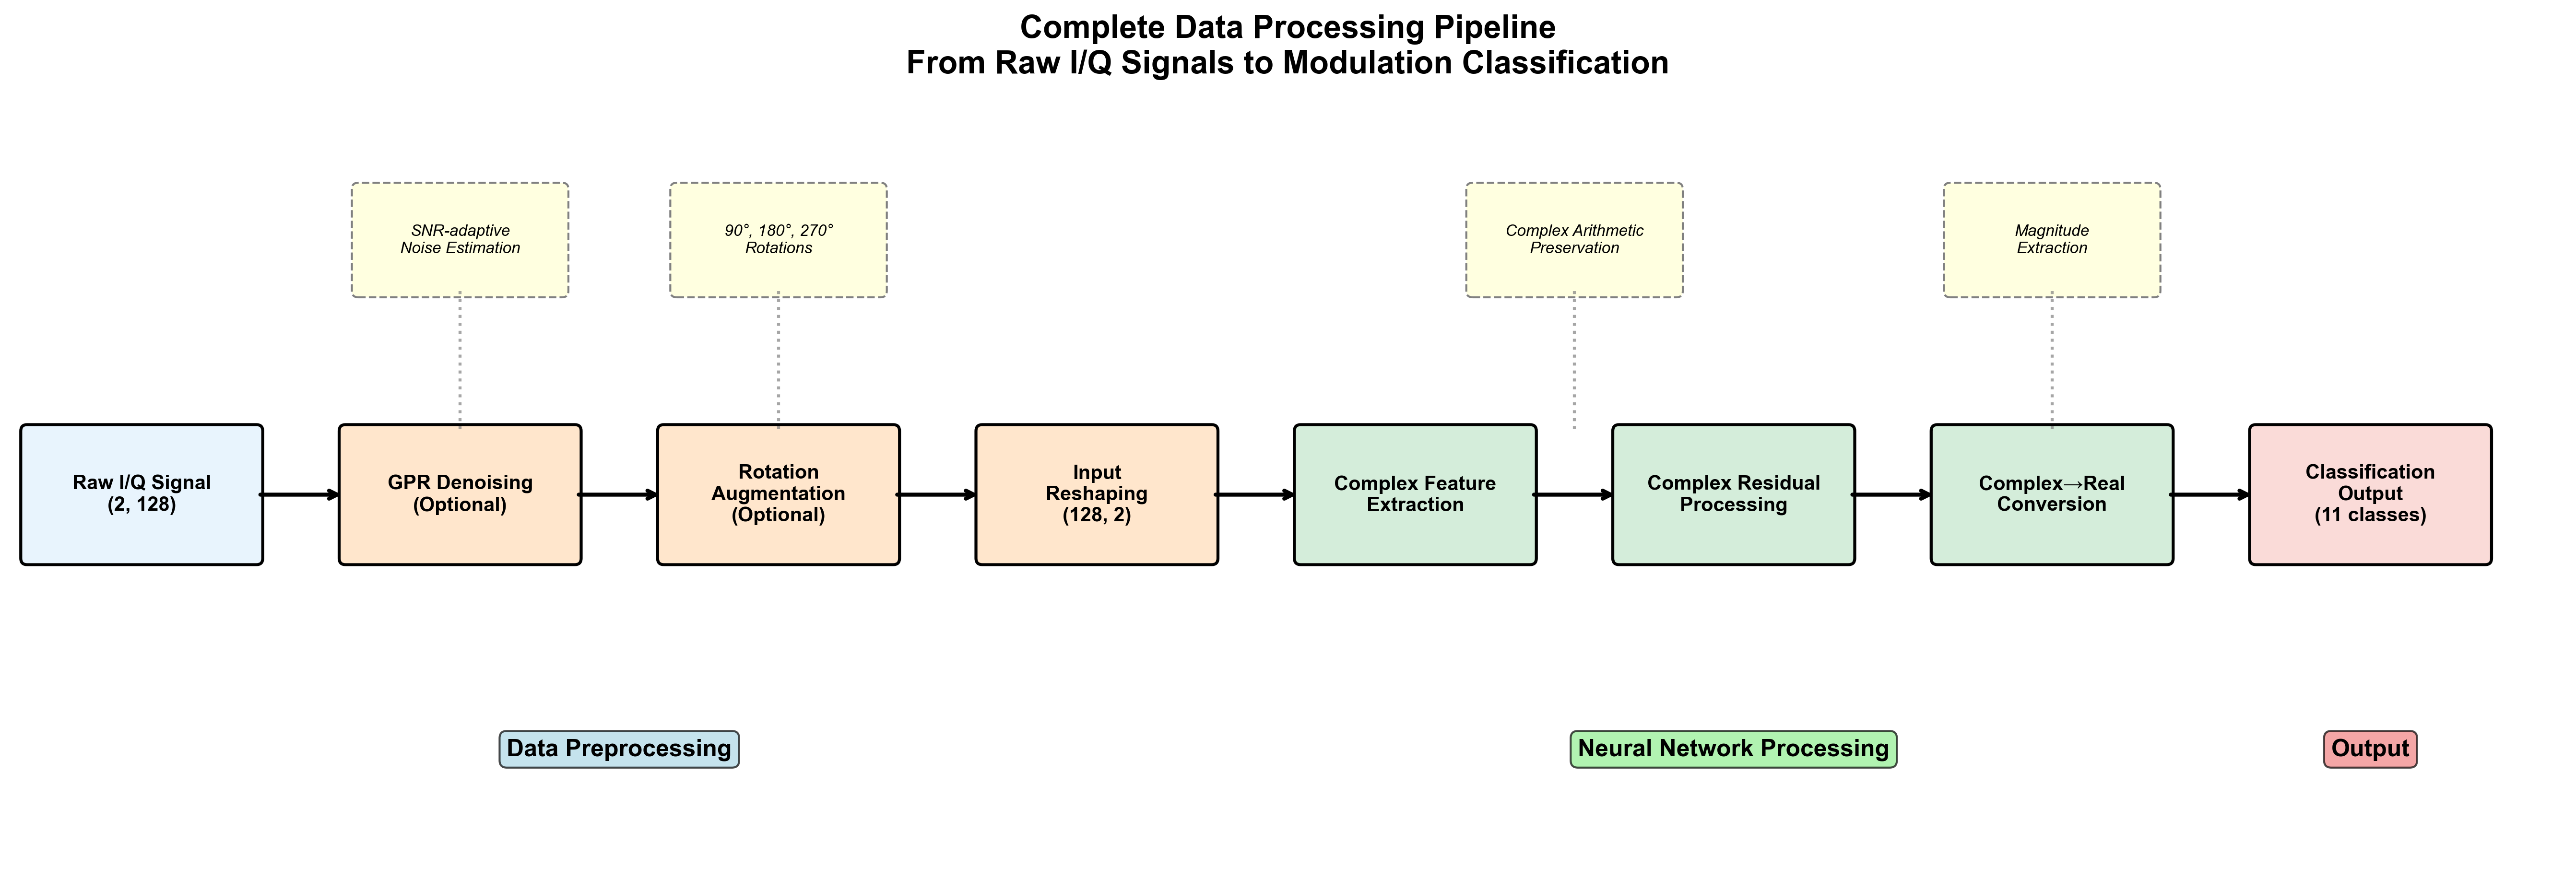
\includegraphics[width=0.9\textwidth]{figure/data_processing_pipeline.png}
\caption{完整的数据处理流程图。该图展示了从原始I/Q信号输入到最终分类输出的整个工作流程,包括GPR去噪、旋转数据增强和复数卷积残差网络处理等阶段。}
\label{fig:data_pipeline}
\end{figure*}

\subsection{数据集与预处理}

本研究采用公开的RML2016.10a数据集进行自动调制分类任务。该数据集包含11种常见的数字和模拟调制类型(8PSK, AM-DSB, AM-SSB, BPSK, CPFSK, GFSK, PAM4, QAM16, QAM64, QPSK, WBFM)。针对每种调制类型,在-20dB到+18dB的信噪比(SNR)范围内,以2dB为步长生成信号样本,共涵盖20个不同的信噪比水平。每个信号样本由128个复数I/Q采样点组成,在数据集中以长度为256的实值向量形式存储。

数据预处理流程遵循标准的机器学习数据处理实践。原始数据集以结构化格式存储,每个样本都与其对应的调制类型和信噪比值相关联。数据集采用分层抽样策略进行划分,以确保在训练集、验证集和测试集中,调制类型和信噪比条件的分布均匀。具体的划分比例为:72\%用于训练集,8\%用于验证集,剩余20\%用于测试集。


\subsection{高斯过程回归去噪}

为提升模型在低信噪比(SNR)条件下的分类性能,本研究引入了一种基于高斯过程回归(GPR)的自适应去噪方法。在实际无线通信系统中,接收信号常受到加性高斯白噪声(AWGN)的干扰,其中 $w[n] \sim \mathcal{CN}(0, \sigma_n^2)$ 表示方差为 $\sigma_n^2$ 的复高斯白噪声。GPR作为一种非参数贝叶斯方法,能够有效建模信号的潜在结构并抑制此类AWGN干扰。

GPR去噪的关键在于对噪声水平的精确估计,这通过GPR模型中的 $\alpha$ 参数(即单分量噪声方差 $\sigma_n^2$)来实现。对于接收到的含噪信号 $r[n]=r_I[n]+jr_Q[n]$,其平均功率定义为 $P_r = \mathbb{E}[|r[n]|^2]$。在实践中,若有 $M$ 个离散时间样本,则通过对这些接收信号样本 $r[k]$(其中 $k=0, \ldots, M-1$)的瞬时功率 $(r_I[k]^2 + r_Q[k]^2)$求和并取平均来估计此平均功率:
\begin{equation}
P_r = \frac{1}{M}\sum_{k=0}^{M-1}(r_I[k]^2+r_Q[k]^2)
\end{equation}

假设原始无噪信号 $s[n]$ 的功率为 $P_s = \mathbb{E}[|s[n]|^2]$,噪声 $w[n]$ 的功率为 $P_w = \mathbb{E}[|w[n]|^2]$。若信号与噪声不相关,则接收信号的总平均功率为:
\begin{equation}
P_r = P_s + P_w
\end{equation}

信噪比(SNR)定义为原始信号功率与噪声功率之比,其线性值为 $\mathrm{SNR}_{\text{linear}} = P_s/P_w$,对应的分贝(dB)值为 $\mathrm{SNR}_{\text{dB}} = 10\log_{10}(\mathrm{SNR}_{\text{linear}})$。
利用该定义,可得 $P_s = \mathrm{SNR}_{\text{linear}} \cdot P_w$。将其代入总功率关系式,有 $P_r = \mathrm{SNR}_{\text{linear}} \cdot P_w + P_w = P_w(\mathrm{SNR}_{\text{linear}} + 1)$。
因此,噪声功率可由测量到的信号功率 $P_r$ 和给定的SNR计算得出:
\begin{equation}
P_w = \frac{P_r}{\mathrm{SNR}_{\text{linear}} + 1} = \frac{P_r}{10^{\mathrm{SNR}_{\text{dB}}/10} + 1}
\end{equation}
对于复高斯白噪声 $w[n]=w_I[n]+jw_Q[n]$,其中同相分量 $w_I[n]$ 和正交分量 $w_Q[n]$ 相互独立,且均服从均值为零、方差为 $\sigma_n^2$ 的正态分布,即 $w_I[n],w_Q[n]\sim\mathcal{N}(0,\sigma_n^2)$。其总噪声功率定义为:
\begin{equation}
P_w=\mathbb{E}[|w[n]|^2]
=\mathbb{E}[w_I[n]^2]+\mathbb{E}[w_Q[n]^2]
=2\sigma_n^2
\end{equation}
由此可得,单个分量的噪声方差为:
\begin{equation}
\sigma_n^2=\frac{P_w}{2}
\end{equation}
噪声标准差为:
\begin{equation}
\sigma_n=\sqrt{\frac{P_w}{2}}
\end{equation}
结合公式(6) $P_w=\frac{P_r}{10^{\mathrm{SNR}_{\mathrm{dB}}/10}+1}$,可进一步得到:
\begin{equation}
\sigma_n=\sqrt{\frac{P_r}{2\bigl(10^{\mathrm{SNR}_{\mathrm{dB}}/10}+1\bigr)}}
\end{equation}
\label{eq:sigma_n_calc}
此 $\sigma_n^2$ 即为GPR模型中设置的噪声水平参数 $\alpha$。

模型采用径向基函数(RBF)、Matern核和有理二次核函数来描述信号的平滑特性。在去噪过程中,以离散的时间索引 $X=[0,1,\ldots,127]$ 作为输入,同相或正交分量本身为观测目标,通过在协方差矩阵中加入噪声参数 $\alpha=\sigma_n^2$ 来实现噪声抑制。

为适应不同SNR条件下信号平滑度的需求,本研究设计了一种基于SNR的自适应长度尺度(length-scale)策略。在高斯过程回归中,长度尺度参数 $L$ 控制核函数的相关范围,直接影响去噪效果的强弱。对于RBF核函数,其表达式为:
\begin{equation}
k(x_i, x_j) = \sigma_f^2 \exp\left(-\frac{(x_i - x_j)^2}{2L^2}\right)
\end{equation}
其中 $\sigma_f^2$ 为信号方差,$L$ 为长度尺度参数。较大的 $L$ 值意味着距离较远的数据点仍有较强相关性,产生更强的平滑效果;而较小的 $L$ 值则使平滑效果更局部化,允许保留更多的信号细节。

在低SNR条件下,噪声幅度相对较大。此时若采用过大的长度尺度 $L$,将导致以下问题:

\textbf{(1) 信号特征的过度平滑:}当 $L$ 过大时,GPR会将相距较远的信号样本视为强相关,导致真实信号的快速变化(如调制信号中的幅度和相位跳变)被误判为噪声而平滑掉。这种过度平滑会模糊不同调制类型间的特征差异。

\textbf{(2) 时域细节的丢失:}数字调制信号含有重要的时域特征,如符号转换点、瞬时频率变化等。过大的 $L$ 会导致这些细节特征被平滑,降低后续分类网络提取有效特征的能力。

\textbf{(3) 相位信息的损失:}对于相位调制信号(如PSK、QAM),相位的快速变化是关键的识别特征。过度平滑将导致相位信息的丢失,严重影响分类准确率。

基于以上分析,本研究提出一种自适应长度尺度策略:设基础长度尺度为 $L_0$。当 $\mathrm{SNR}\ge0$ dB时,取 $L=L_0$;当 $\mathrm{SNR}<0$ dB时,动态调整如下:
\begin{equation}
L = \max\bigl(L_{\min},\,L_0\bigl(1+\mathrm{SNR}/20\bigr)\bigr)
\end{equation}
其中 $L_{\min}$ 为预设的最小尺度。该策略的核心思想是:随着SNR的降低,逐步减小长度尺度 $L$,从而减弱平滑效果,在去除噪声的同时最大程度地保留有效信号信息。

具体而言,当 $\mathrm{SNR}=-20$ dB时,长度尺度调整为 $L=\max(L_{\min}, L_0 \times 0)=L_{\min}$,此时平滑效果最弱,优先保留信号细节;随着SNR逐渐升高,长度尺度相应增大,平滑效果增强。这种自适应机制确保了在高SNR场景下有足够的去噪效果,而在低SNR场景下,通过减弱平滑强度保留了更多有用的信号特征,实现了去噪性能与信号保真度之间的最优权衡。

去噪后的同相和正交分量被重构为复数信号,作为后续神经网络训练的输入数据。

\subsection{基于旋转的数据增强}

\begin{figure}[htbp]
\centering
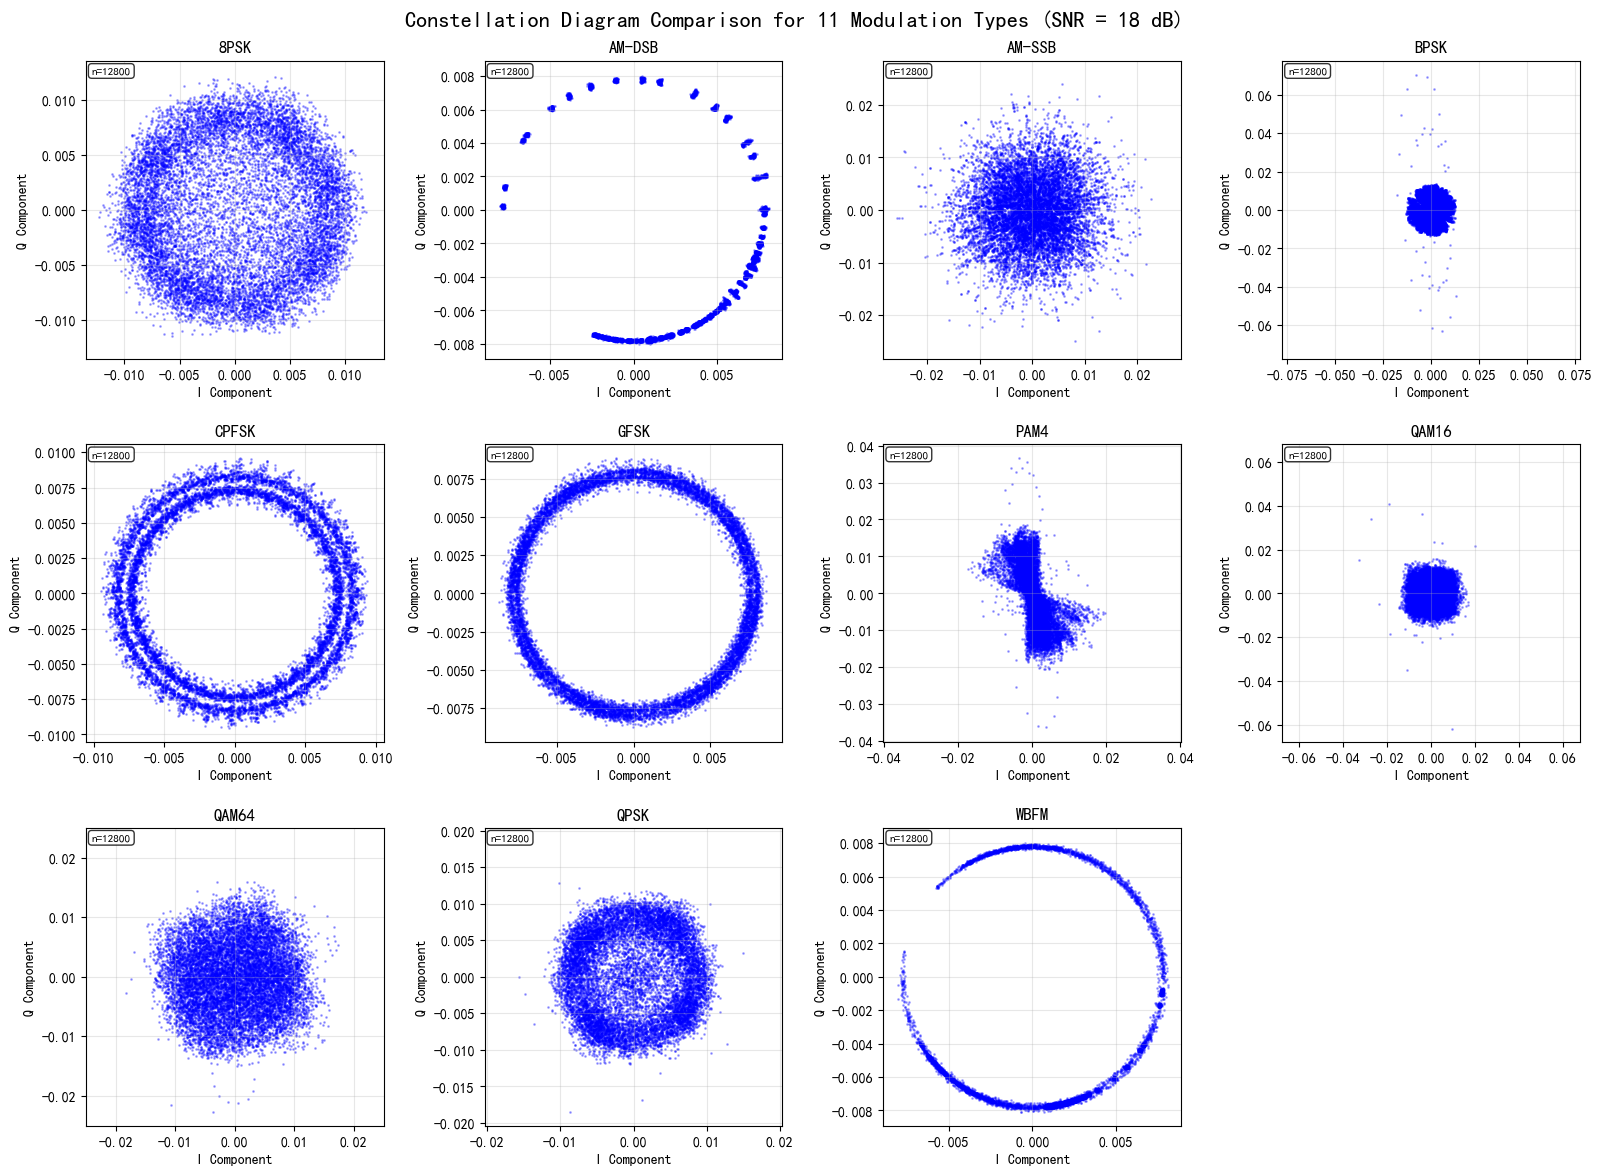
\includegraphics[width=0.45\textwidth]{figure/constellation.png}
\caption{11种调制类型的星座图。该图展示了各种调制方案在I/Q平面上的信号点分布,其旋转对称性是本研究采用旋转数据增强策略的依据。}
\label{fig:constellation}
\end{figure}

考虑到数字调制信号的复数属性以及图~\ref{fig:constellation}中星座图的旋转对称性,本研究采用在复平面上基于旋转的数据增强策略,以增强模型的泛化能力和对相位偏移的鲁棒性~\cite{guo2024ulcnn}。

对于一个复数信号 \(s[n] = s_I[n] + j s_Q[n]\),旋转通过以下数学运算实现。将复数信号表示为向量 \([s_I[n], s_Q[n]]^T\),通过与旋转矩阵 \(R(\theta)\) 相乘来进行旋转:

\begin{equation}
\begin{bmatrix} s'_I[n] \\ s'_Q[n] \end{bmatrix} = \begin{bmatrix} \cos\theta & -\sin\theta \\ \sin\theta & \cos\theta \end{bmatrix} \begin{bmatrix} s_I[n] \\ s_Q[n] \end{bmatrix}
\end{equation}

其中 \(s'_I[n]\) 和 \(s'_Q[n]\) 是旋转后的同相和正交分量,\(\theta\) 是旋转角度。

% \begin{figure*}[htbp]


在实现中,数据增强算法将输入数据张量 \(X_{data}\)(形状为 \((N, 2, L)\),其中 \(N\) 是样本数,\(L\) 是序列长度)和旋转角度 \(\theta_{\text{rad}}\) 作为参数。它首先分离原始的I和Q分量,应用旋转变换矩阵,然后将它们重组为增强后的数据样本。

基于调制类型的对称性,主要使用90° (\(\pi/2\))、180° (\(\pi\)) 和 270° (\(3\pi/2\)) 的旋转,并且该策略仅应用于具有旋转对称性的调制类型(如PSK、QAM)。该方法在保留调制特征的同时,有效地将训练数据集扩大了四倍。通过学习旋转不变的特征表示,模型能够更好地处理由载波相位偏移、多普勒效应等引起的信号旋转。


\subsection{混合ComplexCNN-ResNet架构}

\begin{figure*}[htbp]
\centering
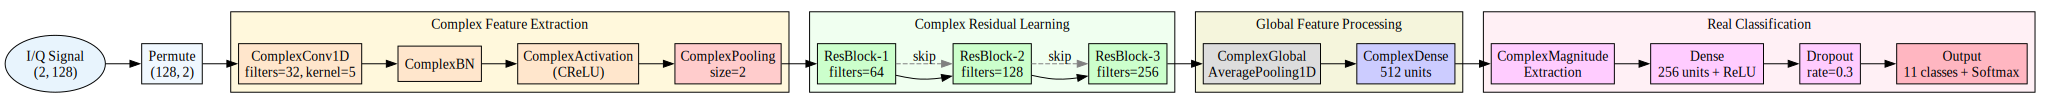
\includegraphics[width=0.85\textwidth]{figure/lightweight_hybrid_model.pdf}
\caption{混合ComplexCNN-ResNet架构的处理流程。该图以框图形式展示了从I/Q信号输入、复数特征提取、残差学习到最终调制分类的完整处理流程,清晰描绘了各模块之间的数据流和处理逻辑。}
\label{fig:lightweight_hybrid_model_flow}
\end{figure*}

\begin{figure*}[htbp]
\centering
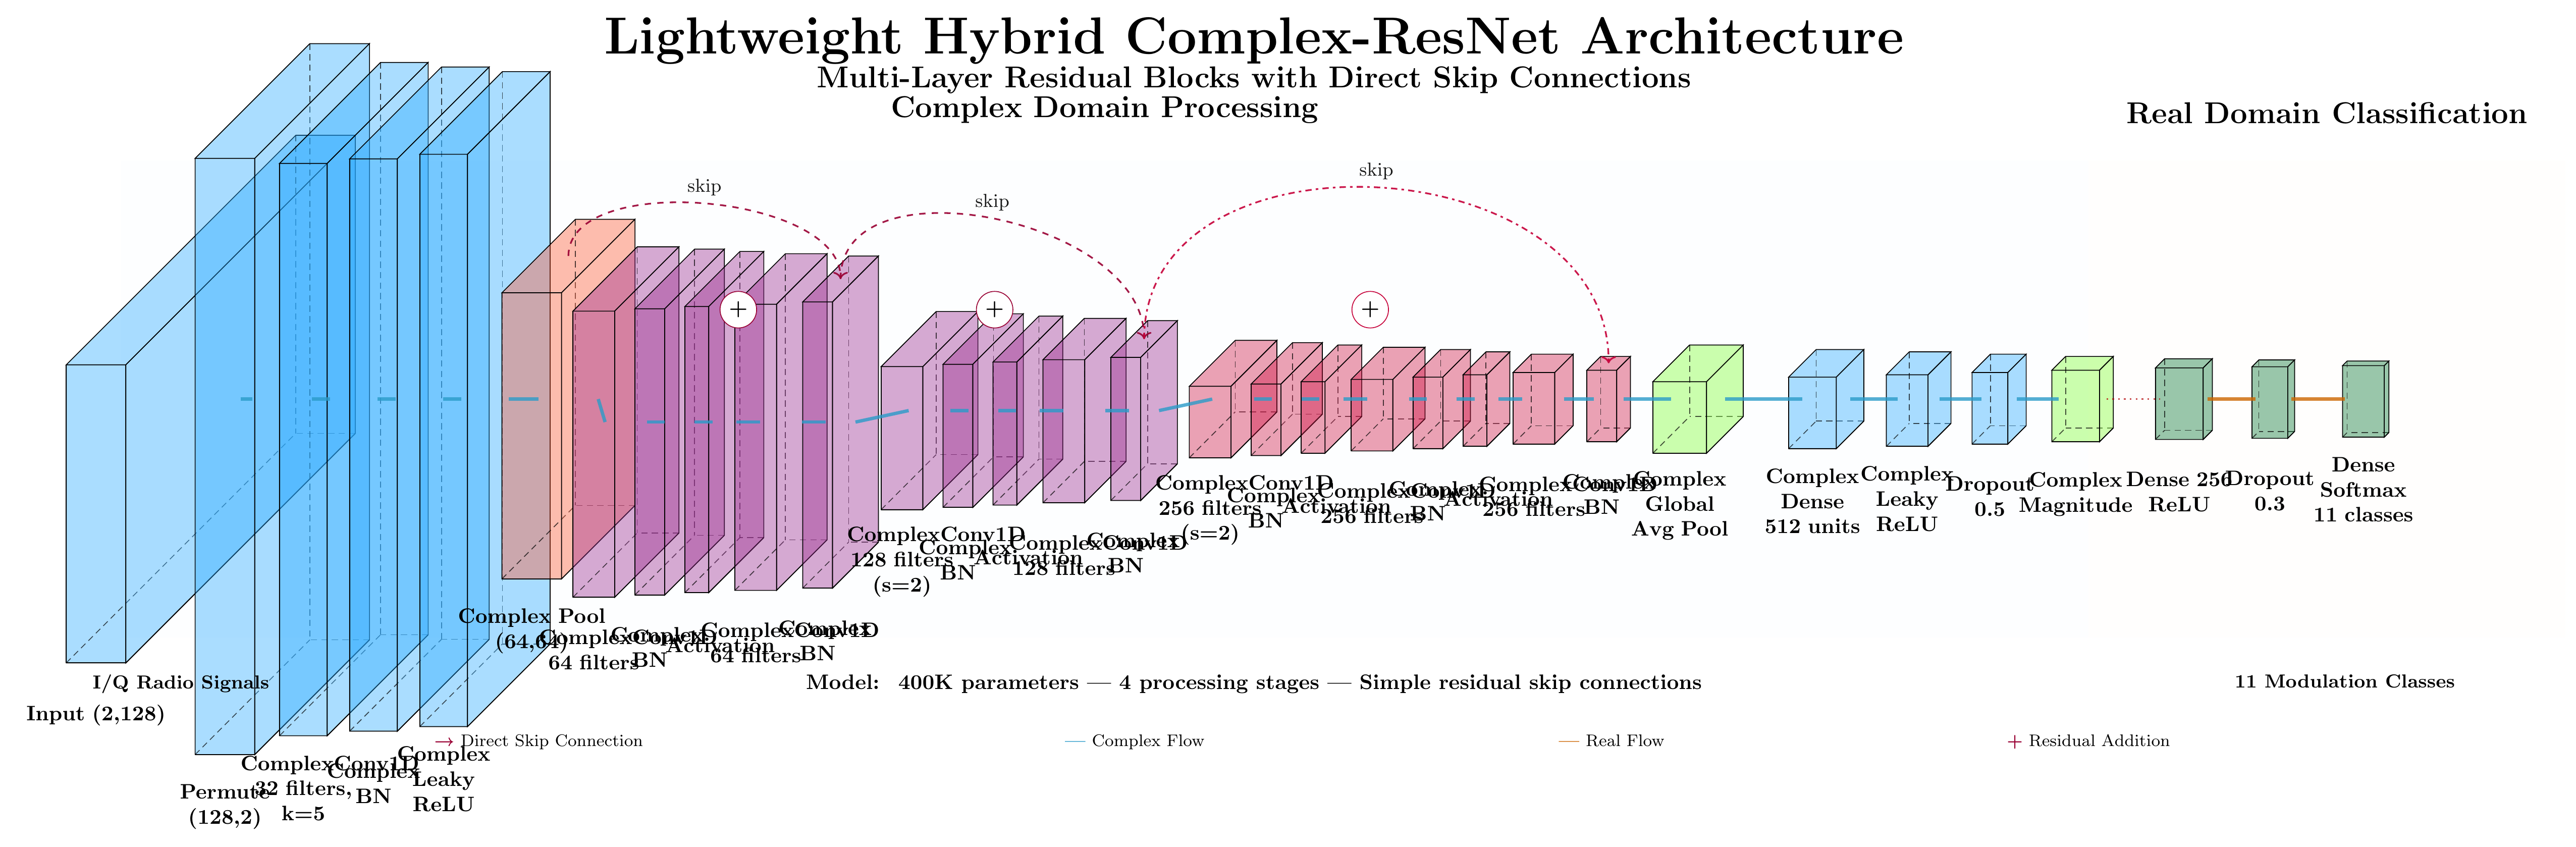
\includegraphics[width=0.9\textwidth]{figure/enhanced_hybrid_model.pdf}
\caption{混合ComplexCNN-ResNet的详细架构。该图展示了从复数输入到最终分类输出的完整数据流,包括复数卷积层、ModReLU激活函数、复数残差块、注意力机制以及复数到实数的转换过程。}
\label{fig:enhanced_hybrid_model}
\end{figure*}

本文提出了一种新颖的混合ComplexCNN-ResNet架构,该架构融合了复数神经网络的快速收敛特性与残差网络的深度特征学习能力,专为无线电信号调制分类任务进行了优化。与传统方法不同,此架构在整个特征提取过程中保持复数域操作,仅在最终分类层转换为实数域,从而最大限度地利用了I/Q信号固有的复数特性。

\textbf{架构设计原则}

混合架构的核心在于将ComplexNN的初始快速收敛能力与ResNet的深度特征学习能力有机地统一起来。ComplexNN在处理复数I/Q数据方面的天然优势,直接保留了信号幅度和相位信息的完整性,而ResNet的残差连接机制有效解决了深度网络中的梯度消失问题,使模型能够学习到更抽象的判别性特征。

该架构采用渐进式特征提取策略,按照复数域处理深度递增的原则组织网络层:

\textbf{复数卷积层设计} 复数卷积层执行真正的复数域卷积运算。对于复数输入 $\mathbf{a} + j\mathbf{b}$ 和复数权重 $\mathbf{c} + j\mathbf{d}$,复数卷积定义为:

\begin{align}
&(\mathbf{a} + j\mathbf{b}) * (\mathbf{c} + j\mathbf{d}) \notag \\
= &(\mathbf{a} * \mathbf{c} - \mathbf{b} * \mathbf{d}) 
+ j(\mathbf{a} * \mathbf{d} + \mathbf{b} * \mathbf{c})
\end{align}

\textbf{ModReLU激活函数} 本文采用ModReLU激活函数以保留复数信号的相位信息。对于复数输入 $z = x + jy$,ModReLU定义为:

\begin{equation}
|z| = \sqrt{x^2 + y^2}
\end{equation}
\begin{equation}
\phi = \arg(z) = \arctan(y/x)
\end{equation}
\begin{equation}
\text{ModReLU}(z) = \text{ReLU}(|z| + b) \cdot e^{j\phi}
\end{equation}

其中 $b$ 是一个可学习的偏置参数。该激活函数对幅度应用ReLU,同时完全保留相位信息,确保复数特征的几何结构不被破坏。

\textbf{复数残差块} 复数残差块是该架构的核心创新,其数学表达式为:
\begin{equation}
\mathbf{H}(z) = \mathbf{F}(z) + z
\end{equation}
其中 $z$ 是复数输入,$\mathbf{F}(z)$ 是学习到的复数残差函数。

基础残差块使用两层结构:

\begin{equation}
h_1 = \text{ModReLU}(\text{CBN}(\text{CConv}(z)))
\end{equation}
\begin{equation}
h_2 = \text{CBN}(\text{CConv}(h_1))
\end{equation}
\begin{equation}
\mathbf{H}(z) = \text{ModReLU}(h_2 + z)
\end{equation}

其中 CBN 表示复数批归一化(Complex Batch Normalization),CConv 表示复数卷积。

\textbf{复数批归一化} 复数批归一化通过白化变换对复数分布进行标准化。对于复数输入 $z = x + jy$,协方差矩阵为:
\begin{equation}
\mathbf{C} = \begin{bmatrix} V_{xx} & V_{xy} \\ V_{xy} & V_{yy} \end{bmatrix}
\end{equation}

白化矩阵 $\mathbf{W}$ 的获取方式如下:
\begin{align}
s &= \sqrt{V_{xx}V_{yy} - V_{xy}^2} \\
t &= \sqrt{V_{xx} + V_{yy} + 2s} \\
\mathbf{W} &= \frac{1}{st}\begin{bmatrix} V_{yy} + s & -V_{xy} \\ -V_{xy} & V_{xx} + s \end{bmatrix}
\end{align}

\textbf{带注意力机制的高级残差块} 高级复数残差块使用三层卷积结构并集成了复数注意力:
\begin{align}
h_1 &= \text{ModReLU}(\text{CBN}(\text{CConv}(z))) \\
h_2 &= \text{ModReLU}(\text{CBN}(\text{CConv}(h_1))) \\
h_3 &= \text{CBN}(\text{CConv}_{1 \times 1}(h_2))
\end{align}

复数注意力权重的计算方式为:
\begin{equation}
\mathbf{A} = \text{Tanh}(\text{CConv}_{1 \times 1}(h_3))
\end{equation}

最终输出为:
\begin{equation}
\mathbf{H}(z) = \text{ModReLU}(h_3 \odot \mathbf{A} + z_{shortcut})
\end{equation}
其中 $\odot$ 表示复数逐元素相乘。

\textbf{全局特征聚合} 复数全局平均池化将时间特征聚合为全局表示:
\begin{equation}
f_{global} = \frac{1}{T} \sum_{t=1}^T z_t
\end{equation}

\textbf{复数到实数转换} 最后,通过提取幅度来转换为实数域:
\begin{equation}
|z| = \sqrt{x^2 + y^2 + \epsilon}
\end{equation}
其中 $\epsilon$ 是一个数值稳定项。

这种混合架构的主要优点包括:(1) 完全保留I/Q信号的复数特性和相位信息;(2) 残差连接确保了深度网络的有效训练;(3) ModReLU激活函数在非线性变换中保持了相位的完整性;(4) 轻量化设计在保持性能的同时显著降低了计算复杂性。通过这种精心设计的混合架构,模型能够充分利用I/Q信号的内在结构特征,实现对不同调制类型的精确分类。


\section{实验设置}

\subsection{训练配置}

本研究的所有实验均在配备Intel Core i9-13900K处理器、NVIDIA GeForce RTX 4090 GPU(24GB GDDR6X显存)和64GB系统内存的高性能工作站上进行。深度学习框架采用TensorFlow 2.17.0和Keras 3.6.0,并使用CUDA 12.4和cuDNN 9.1.1.17进行GPU加速计算。操作系统为Ubuntu 24.04.2 LTS。

\textbf{超参数设置:}
所有模型均采用统一配置进行训练,以确保公平比较。学习率设置为0.001,使用Adam优化器,批处理大小为128。训练过程采用早停机制,若验证集准确率连续30个周期未提升则停止训练,最多训练200个周期。为防止过拟合,在全连接层使用Dropout正则化,丢弃率为0.5。

\textbf{学习率调度:}
采用阶梯式学习率衰减策略。初始学习率为0.001,若验证集准确率在5个周期内未提升,则衰减为当前值的0.5倍,最小学习率设置为1e-6。此调度策略有助于模型在训练后期进行微调。

\textbf{数据划分策略:}
数据集按72\%:8\%:20\%的比例划分为训练集、验证集和测试集,确保每种调制类型和信噪比条件在三个集合中分布均匀。验证集用于超参数调优和模型选择,而测试集仅用于最终性能评估。

\textbf{训练流程:}
为评估改进方法,采用渐进式训练策略:首先训练基线模型,然后依次添加GPR去噪、旋转数据增强和混合架构。每个阶段都独立训练,并记录性能提升。最后,训练包含所有改进的完整模型。

\subsection{评估指标}

本研究采用多维度评估体系,全面分析所提方法的性能。

\textbf{分类准确率:}
主要评估指标为总体分类准确率,定义为正确分类的样本数与总样本数之比:
\begin{equation}
\text{准确率} = \frac{N_{correct}}{N_{total}} \times 100\%
\end{equation}

\textbf{信噪比条件下的性能分析:}
为评估模型在不同噪声条件下的鲁棒性,将测试集根据信噪比范围划分为三个子集:低信噪比(-20dB至-2dB)、中信噪比(0dB至8dB)和高信噪比(10dB至18dB)。对每个子集分别计算准确率。

\textbf{混淆矩阵分析:}
使用混淆矩阵分析各调制类型的分类性能,计算每个类别的精确率(Precision)、召回率(Recall)和F1分数(F1-score):

\begin{equation}
\text{精确率} = \frac{TP}{TP + FP}
\end{equation}
\begin{equation}
\text{召回率} = \frac{TP}{TP + FN}
\end{equation}
\begin{equation}
\text{F1分数} = \frac{2 \times \text{精确率} \times \text{召回率}}{\text{精确率} + \text{召回率}}
\end{equation}

其中TP、FP和FN分别代表真正例、假正例和假负例的数量。

\section{结果与分析}

\subsection{基线性能比较}

为验证所提混合架构的有效性,我们首先在RML2016.10a数据集上评估了多种基线模型的性能,包括全连接神经网络(FCNN)、一维卷积神经网络(CNN1D)、二维卷积神经网络(CNN2D)、残差网络(ResNet)、Transformer以及复数卷积神经网络(ComplexCNN)。

表~\ref{tab:baseline_comparison} 展示了各种基线模型在相同训练条件下的性能对比。实验结果表明,不同架构在分类性能上存在显著差异。ResNet架构因其残差连接机制有效缓解了梯度消失问题,在深度网络训练中表现出优异的收敛特性,取得了55.37\%的分类准确率。ComplexCNN在处理复数I/Q信号方面具有天然优势,能更好地保留信号的相位信息,获得了57.11\%的准确率。

\begin{table}[!htbp]
\centering
\caption{基线模型性能对比}
\label{tab:baseline_comparison}
\begin{tabular}{@{}cc@{}}
\toprule
模型架构 & 准确率 (\%) \\
\midrule
FCNN & 42.65 \\
CNN2D & 47.31 \\
Transformer & 47.86 \\
CNN1D & 54.94 \\
ResNet & 55.37 \\
ComplexCNN & 57.11 \\
\bottomrule
\end{tabular}
\end{table}

\begin{figure}[htbp]
\centering
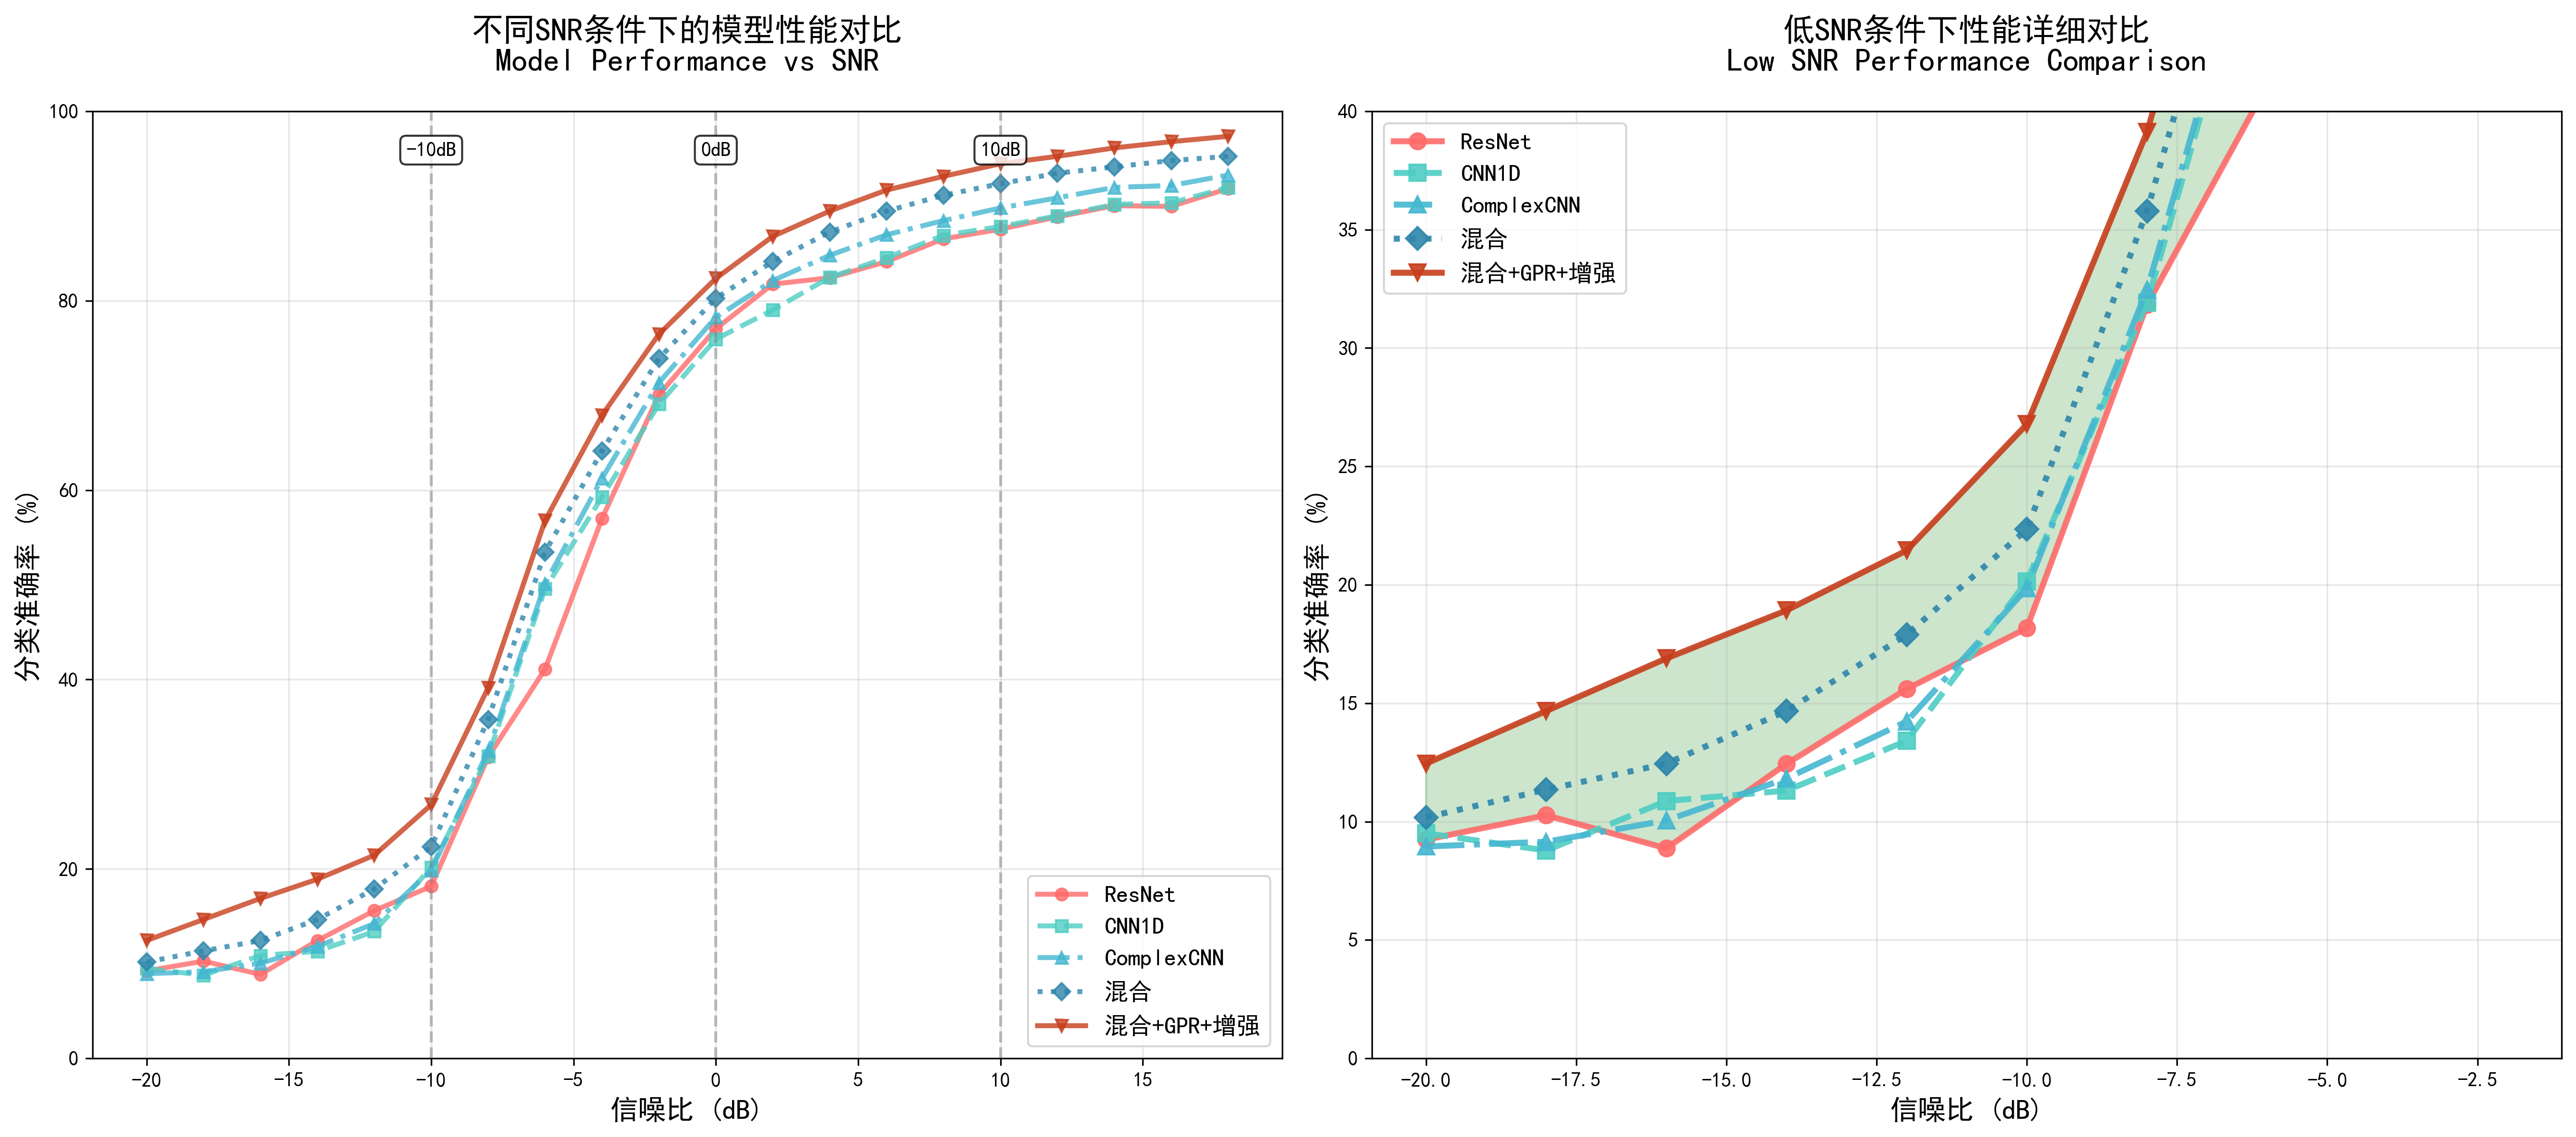
\includegraphics[width=0.45\textwidth]{figure/snr_performance_comparison.pdf}
\caption{不同模型在不同信噪比条件下的性能比较。图中展示了五种模型(CNN1D、ResNet、ComplexCNN、混合架构、混合架构+GPR+增强)在不同信噪比条件下的分类准确率曲线。}
\label{fig:snr_performance}
\end{figure}

图~\ref{fig:snr_performance} 展示了不同基线模型在各种信噪比条件下的性能曲线。可以观察到,所有模型在低信噪比条件下性能均出现显著下降,但ComplexCNN和ResNet在中高信噪比条件下表现相对稳定,这为我们的混合架构设计提供了重要参考。

基于这些基线实验的结果与分析,我们设计了一种融合ResNet的残差学习能力和ComplexCNN的复数处理优势的混合架构。该混合模型结合GPR去噪和旋转数据增强技术,最终在RML2016.10a数据集上实现了65.38\%的分类准确率,相较于最优的单一基线架构(ComplexCNN),实现了8.27个百分点的显著提升。

\begin{figure}[htbp]
\centering
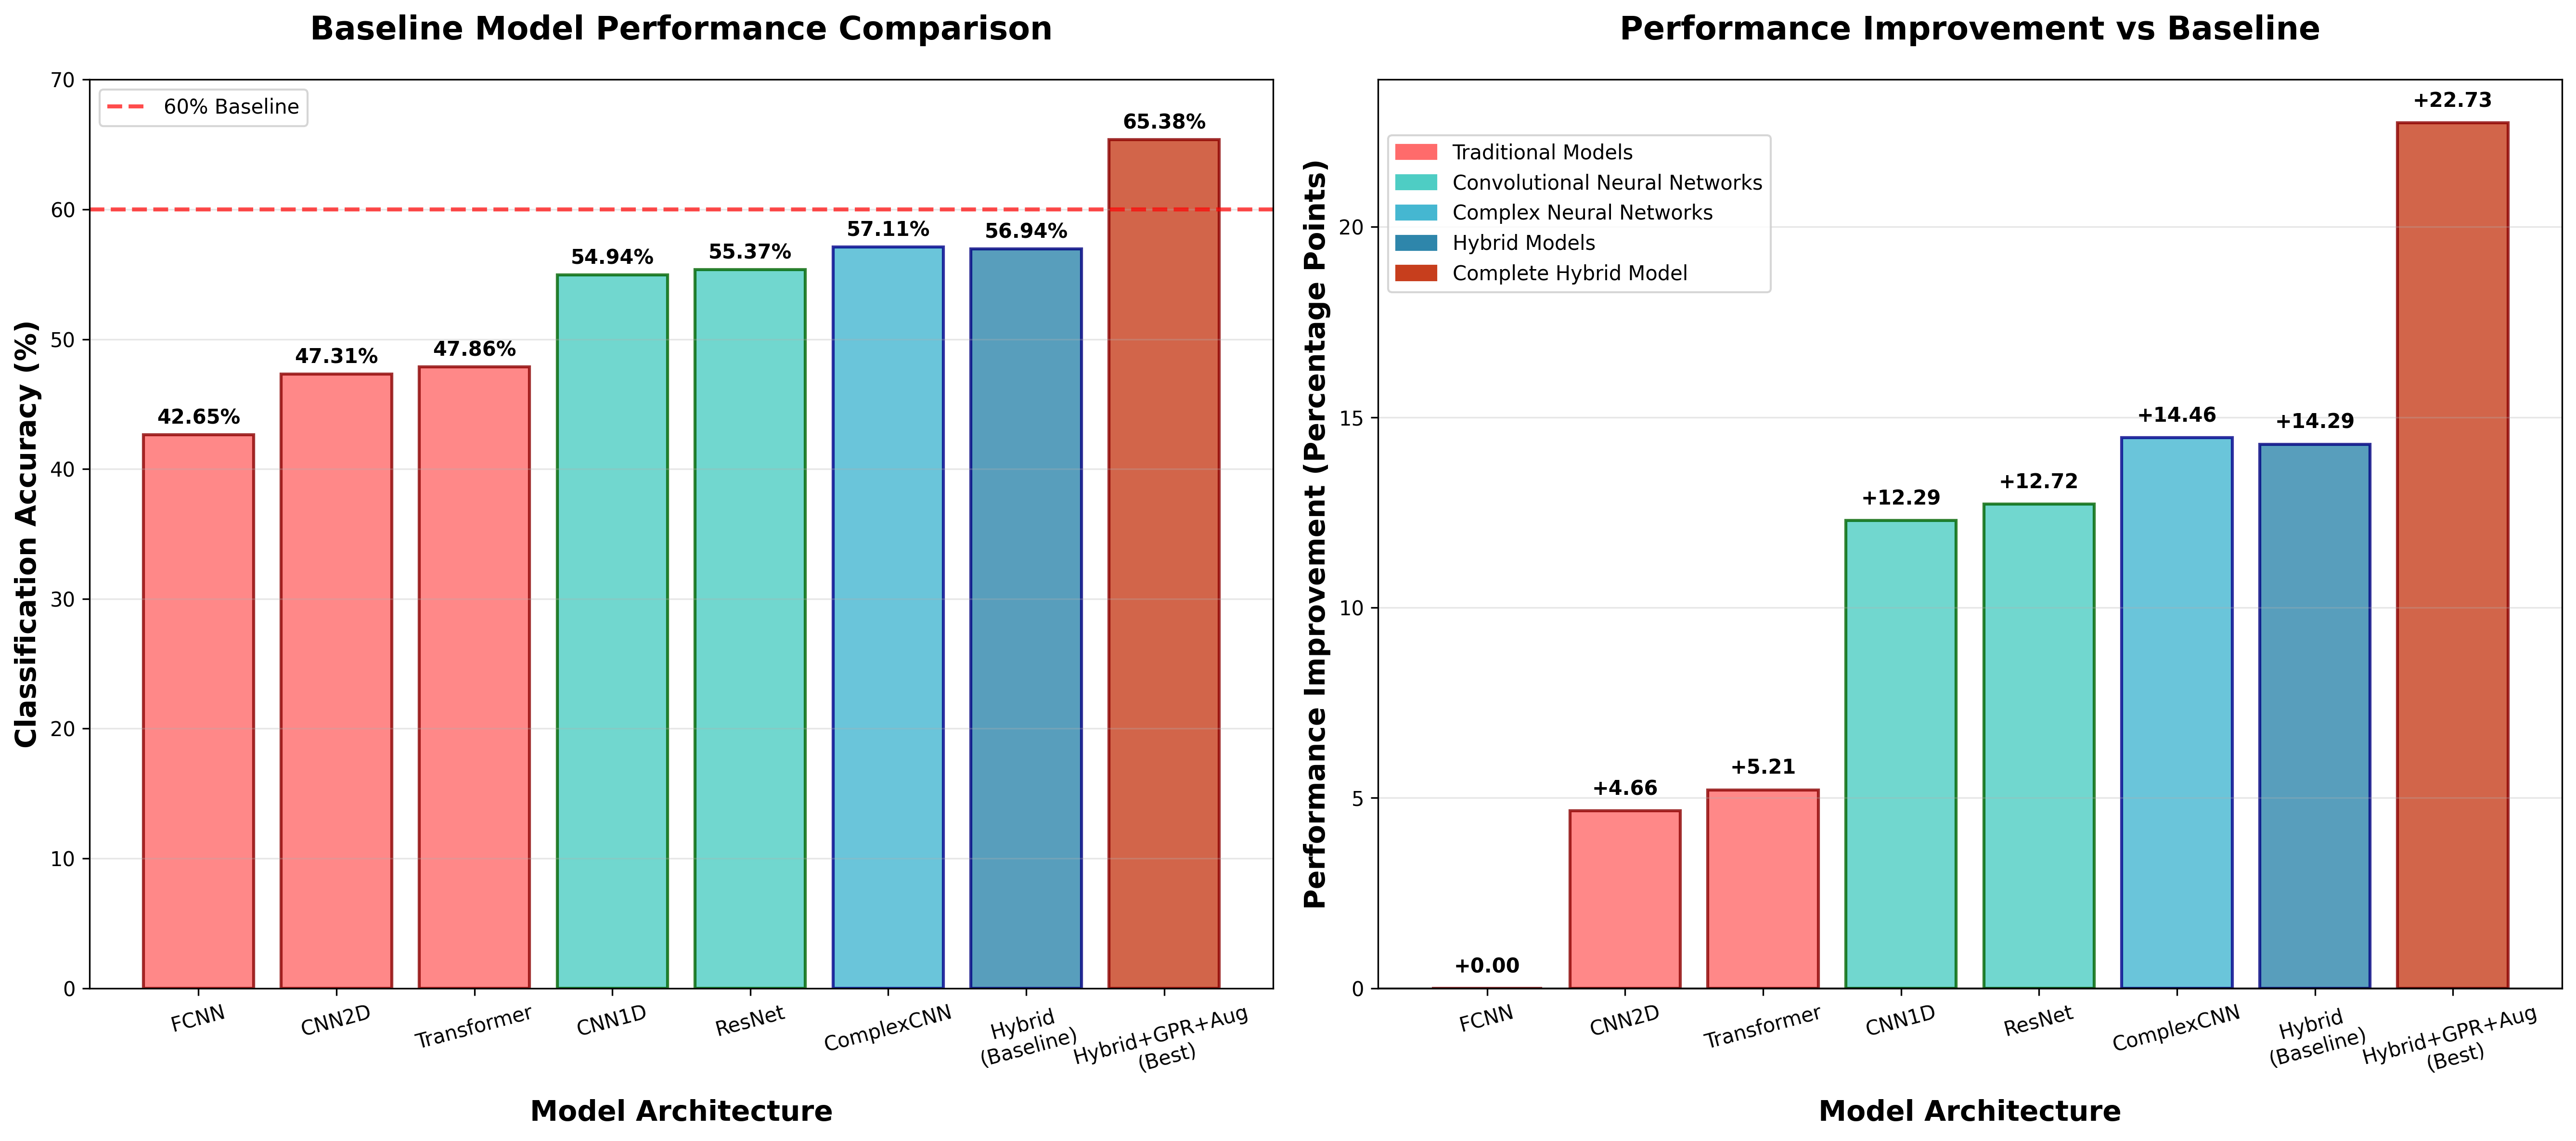
\includegraphics[width=0.45\textwidth]{figure/baseline_model_comparison.pdf}
\caption{不同模型架构的性能比较分析。该图展示了混合架构与传统基线模型在分类准确率、模型参数量和推理时间等关键指标上的综合对比。}
\label{fig:model_comparison}
\end{figure}

\subsection{高斯过程回归去噪的影响}
GPR去噪技术在提升模型性能方面发挥了显著作用,在所有信噪比条件下均表现出明显改善。图~\ref{fig:constellation_denoising} 展示了GPR去噪前后信号质量的对比,清晰地说明了噪声得到了有效抑制。

表~\ref{tab:gpr_impact} 详细分析了GPR去噪在不同信噪比范围对分类准确率的影响。实验结果显示,GPR去噪在低信噪比条件(-20dB至-8dB)下带来了7.25个百分点的性能提升,在中信噪比条件(-6dB至4dB)下提升了5.12个百分点,在高信噪比条件(6dB至18dB)下提升了5.07个百分点。总体而言,GPR去噪使混合架构的准确率从56.94\%提升至62.80\%,实现了5.86个百分点的显著改善。这一结果表明,GPR去噪技术在所有信噪比范围内均提供了稳定且可观的性能增益,其中在低信噪比条件下的绝对提升最大,凸显了去噪技术在恶劣信道环境中的重要性。

\begin{table}[!htbp]
\centering
\caption{GPR去噪在不同信噪比范围的影响}
\label{tab:gpr_impact}
\begin{threeparttable}
\begin{tabular}{@{}cccc@{}}
\toprule
信噪比范围 & 去噪前 (\%) & 去噪后 (\%) & 提升 (\%) \\
\midrule
低信噪比$^{a}$ & 15.14 & 22.40 & +7.25 \\
中信噪比$^{b}$ & 73.58 & 78.70 & +5.12 \\
高信噪比$^{c}$ & 84.15 & 89.23 & +5.07 \\
总体 & 56.94 & 62.80 & +5.86 \\
\bottomrule
\end{tabular}
\begin{tablenotes}
\footnotesize
\item[$^{a}$] 低信噪比: -20dB 至 -8dB
\item[$^{b}$] 中信噪比: -6dB 至 4dB  
\item[$^{c}$] 高信噪比: 6dB 至 18dB
\end{tablenotes}
\end{threeparttable}
\end{table}

\begin{figure}[htbp]
\centering
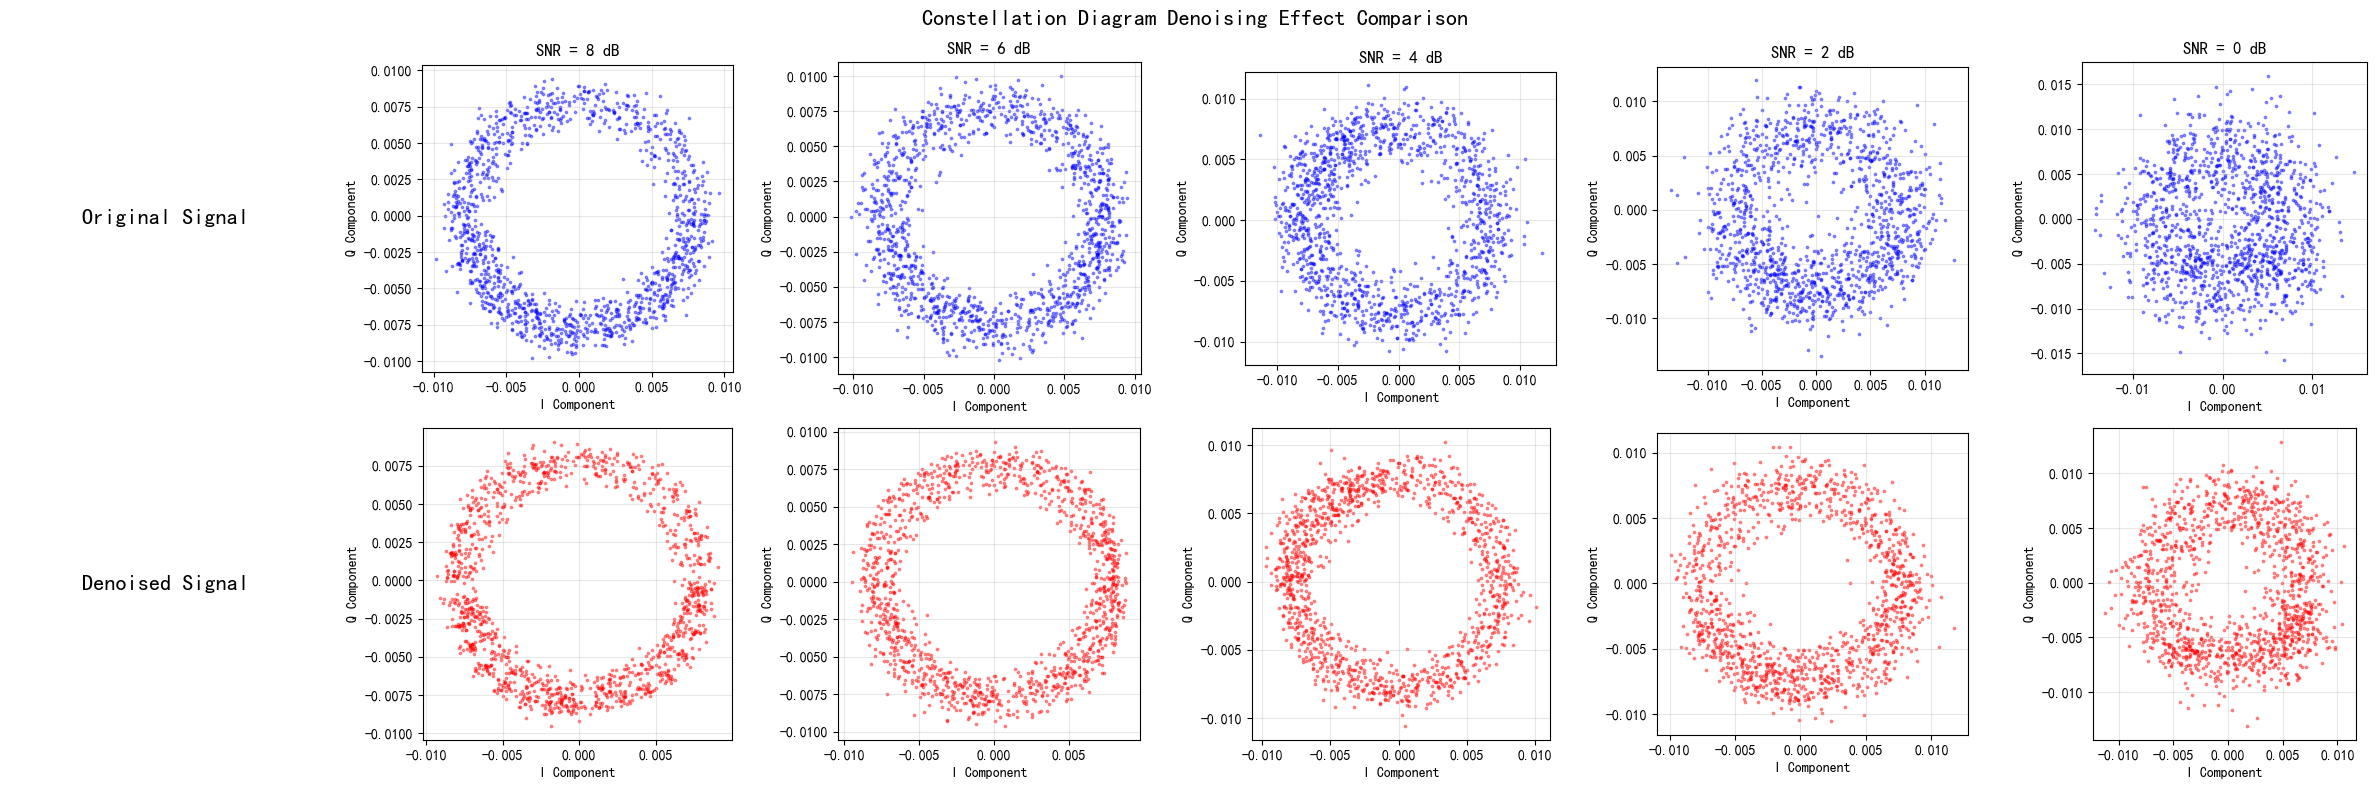
\includegraphics[width=0.45\textwidth]{figure/constellation_denoising.png}
\caption{CPFSK调制类型在0至8dB信噪比条件下星座图的去噪效果。}
\label{fig:constellation_denoising}
\end{figure}

图~\ref{fig:constellation_denoising} 展示了CPFSK调制类型在0至8dB信噪比条件下星座图的去噪效果。从图中可以看出,GPR去噪在有效保留信号结构特征的同时,显著降低了噪声影响,为后续的深度学习分类奠定了良好基础。

表~\ref{tab:gpr_detailed_snr} 提供了对GPR去噪效果更详细的分析,展示了在每个特定信噪比值下分类准确率的变化。从表中可以清晰地看到,GPR去噪在低信噪比条件下带来了更大的提升。随着信噪比的增加,提升幅度呈现出复杂的变化规律。在极低信噪比条件(-20dB至-18dB)下,提升相对较小(1.03\%至1.54\%);而在中低信噪比条件(-12dB至-10dB)下,提升效果达到峰值,分别取得了11.53\%和14.90\%的显著增益。在中信噪比条件(0dB)下,准确率从79.43\%提升至83.17\%,提升了3.74\%;在高信噪比条件(18dB)下,准确率从83.87\%提升至88.98\%,提升了5.11\%。这一趋势表明,GPR去噪在中低信噪比条件下效果最为显著,在极低和高信噪比条件下的提升相对温和,与信号处理中的理论预期相符。

\begin{table}[!htbp]
\centering
\caption{GPR去噪在各信噪比水平的详细影响}
\label{tab:gpr_detailed_snr}
\begin{threeparttable}
\begin{tabular}{@{}cccc@{}}
\toprule
信噪比 (dB) & 基线 (\%) & 基线+GPR (\%) & 提升 (\%) \\
\midrule
-20 & 8.93 & 9.96 & +1.03 \\
-18 & 8.68 & 10.22 & +1.54 \\
-16 & 9.85 & 12.69 & +2.84 \\
-14 & 11.08 & 17.32 & +6.24 \\
-12 & 12.65 & 24.18 & +11.53 \\
-10 & 20.15 & 35.05 & +14.90 \\
-8 & 34.66 & 47.36 & +12.70 \\
-6 & 54.86 & 61.21 & +6.35 \\
-4 & 64.02 & 70.84 & +6.82 \\
-2 & 75.66 & 80.89 & +5.23 \\
0 & 79.43 & 83.17 & +3.74 \\
2 & 82.96 & 87.07 & +4.11 \\
4 & 84.56 & 89.00 & +4.44 \\
6 & 83.93 & 89.38 & +5.45 \\
8 & 83.17 & 89.10 & +5.93 \\
10 & 84.73 & 89.85 & +5.12 \\
12 & 85.81 & 90.31 & +4.50 \\
14 & 85.31 & 88.81 & +3.50 \\
16 & 82.25 & 88.15 & +5.90 \\
18 & 83.87 & 88.98 & +5.11 \\
\bottomrule
\end{tabular}
\begin{tablenotes}
\item[] \textbf{注:} 表中“基线”指混合架构,“基线+GPR”指添加了GPR去噪的混合架构。
\end{tablenotes}
\end{threeparttable}
\end{table}



\subsection{基于旋转的数据增强效果}

在复平面上基于旋转的数据增强策略显著提升了模型的泛化能力和对相位偏移的鲁棒性。该技术利用了数字调制信号星座图的旋转对称性,通过90°、180°和270°的旋转变换,将训练数据集扩展至原始大小的四倍。

表~\ref{tab:data_augmentation_results} 展示了数据增强对不同调制类型分类性能的影响。实验结果表明,旋转数据增强对QAM类调制(QAM16, QAM64)和部分PSK类调制的性能提升最为显著。QAM16的准确率从基线的46\%大幅提升至68\%,提升了22个百分点;QAM64从54\%提升至75\%,增加了21个百分点。对于8PSK,准确率从72\%上升至82\%,增加了10个百分点;BPSK从72\%提升至80\%,增加了8个百分点。GFSK也表现出显著改善,从76\%提升至88\%,增加了12个百分点。总体而言,旋转数据增强使混合架构的准确率从56.94\%提升至60.72\%,实现了3.78个百分点的显著改善。

\begin{table}[!htbp]
\centering
\caption{数据增强对各种调制类型的影响}
\label{tab:data_augmentation_results}
\begin{tabular}{@{}cccc@{}}
\toprule
调制方式 & 基线 (\%) & 增强后 (\%) & 提升 (\%) \\
\midrule
8PSK     & 72  & 82  & +10 \\
AM-DSB   & 54  & 57  & +3  \\
AM-SSB   & 27  & 26  & -1  \\
BPSK     & 72  & 80  & +8  \\
CPFSK    & 82  & 88  & +6  \\
GFSK     & 76  & 88  & +12 \\
PAM4     & 92  & 93  & +1  \\
QAM16    & 46  & 68  & +22 \\
QAM64    & 54  & 75  & +21 \\
QPSK     & 84  & 75  & -9  \\
WBFM     & 82  & 85  & +3  \\
\bottomrule
\end{tabular}
\end{table}

\begin{figure}[htbp]
\centering
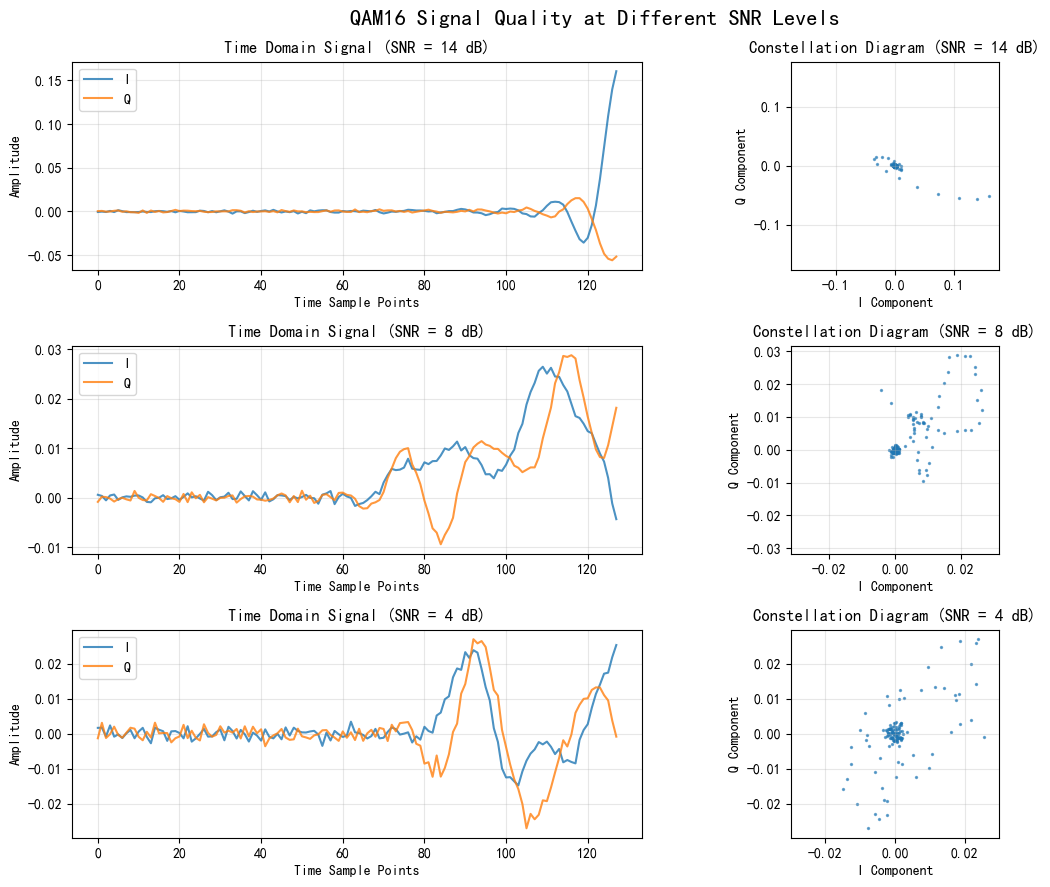
\includegraphics[width=0.45\textwidth]{figure/QAM16_rotation.png}
\caption{QAM16信号的I/Q通道图与星座图。}
\label{fig:rotation_augmentation}
\end{figure}

图~\ref{fig:rotation_augmentation} 展示了部分QAM16信号的I/Q通道图和星座图。从星座图中可以观察到,单个信号具有明确的方向性。旋转变换可以增强信号在不同方向上的信息,为模型提供更丰富的训练样本。这种增强策略在处理实际通信环境中由载波相位偏移、本振频率偏差等因素引起的信号旋转问题时尤为有效。

\subsection{混合架构性能}

所提出的混合ComplexCNN-ResNet架构在RML2016.10a数据集上取得了显著的性能提升,最终分类准确率达到65.38\%。这相比于最优单一基线架构ComplexCNN的57.11\%准确率,提升了8.27个百分点。

图~\ref{fig:method_comparison} 和 表~\ref{tab:hybrid_performance} 展示了混合架构与现有先进方法的详细性能对比。对结果的深入分析揭示了模型性能的显著转变。最初,基线模型与最先进方法之间存在巨大的性能差距。然而,系统性地集成高斯过程回归(GPR)去噪和基于旋转的数据增强技术,从根本上改变了性能格局。增强版的ResNet、ComplexCNN以及混合的ComplexCNN-ResNet架构都达到了与现有先进方法相当或超越的性能水平。

对图~\ref{fig:method_comparison} 的深入研究揭示了有趣的架构动态,这激发了我们的混合设计方法。最初,在基线配置中,ComplexCNN表现出优于ResNet的分类准确率。然而,当应用GPR去噪和基于旋转的数据增强后,出现了显著的性能反转:在这些增强条件下,ResNet开始超越ComplexCNN。这一现象表明,ResNet更深的残差结构具有更强的能力从GPR去噪后的数据中提取有意义的模式,有效地利用了预处理技术所提供的信号质量提升。认识到这种互补行为,我们开发了混合ComplexCNN-ResNet架构,以利用两种方法的优势。虽然基线混合模型的性能略低于独立的ComplexCNN(但仍具竞争力),但GPR去噪和旋转数据增强的集成使混合架构能够超越增强后的ComplexCNN(63.41\%)和增强后的ResNet(64.37\%),最终达到了我们65.38\%的最佳性能,并超过了之前64.59\%的最先进基准。

实验结果表明,所提出的混合方法在准确率、参数效率和训练稳定性等多个维度上均优于现有方法。最值得注意的是,优化后的混合ComplexCNN-ResNet架构成功超越了AbFTNet(64.59\%)所建立的先前最先进性能,达到了65.38\%的新基准准确率,并确立了其在自动调制分类领域新的最先进(SOTA)方法的地位。与Ultra Lite CNN(ULCNN)的62.47\%准确率相比,我们的方法提升了2.91个百分点;与AMC-NET的62.51\%相比,提升了2.87个百分点;与先前的SOTA方法AbFTNet的64.59\%相比,取得了0.79个百分点的有意义提升。

\begin{figure}[htbp]
\centering
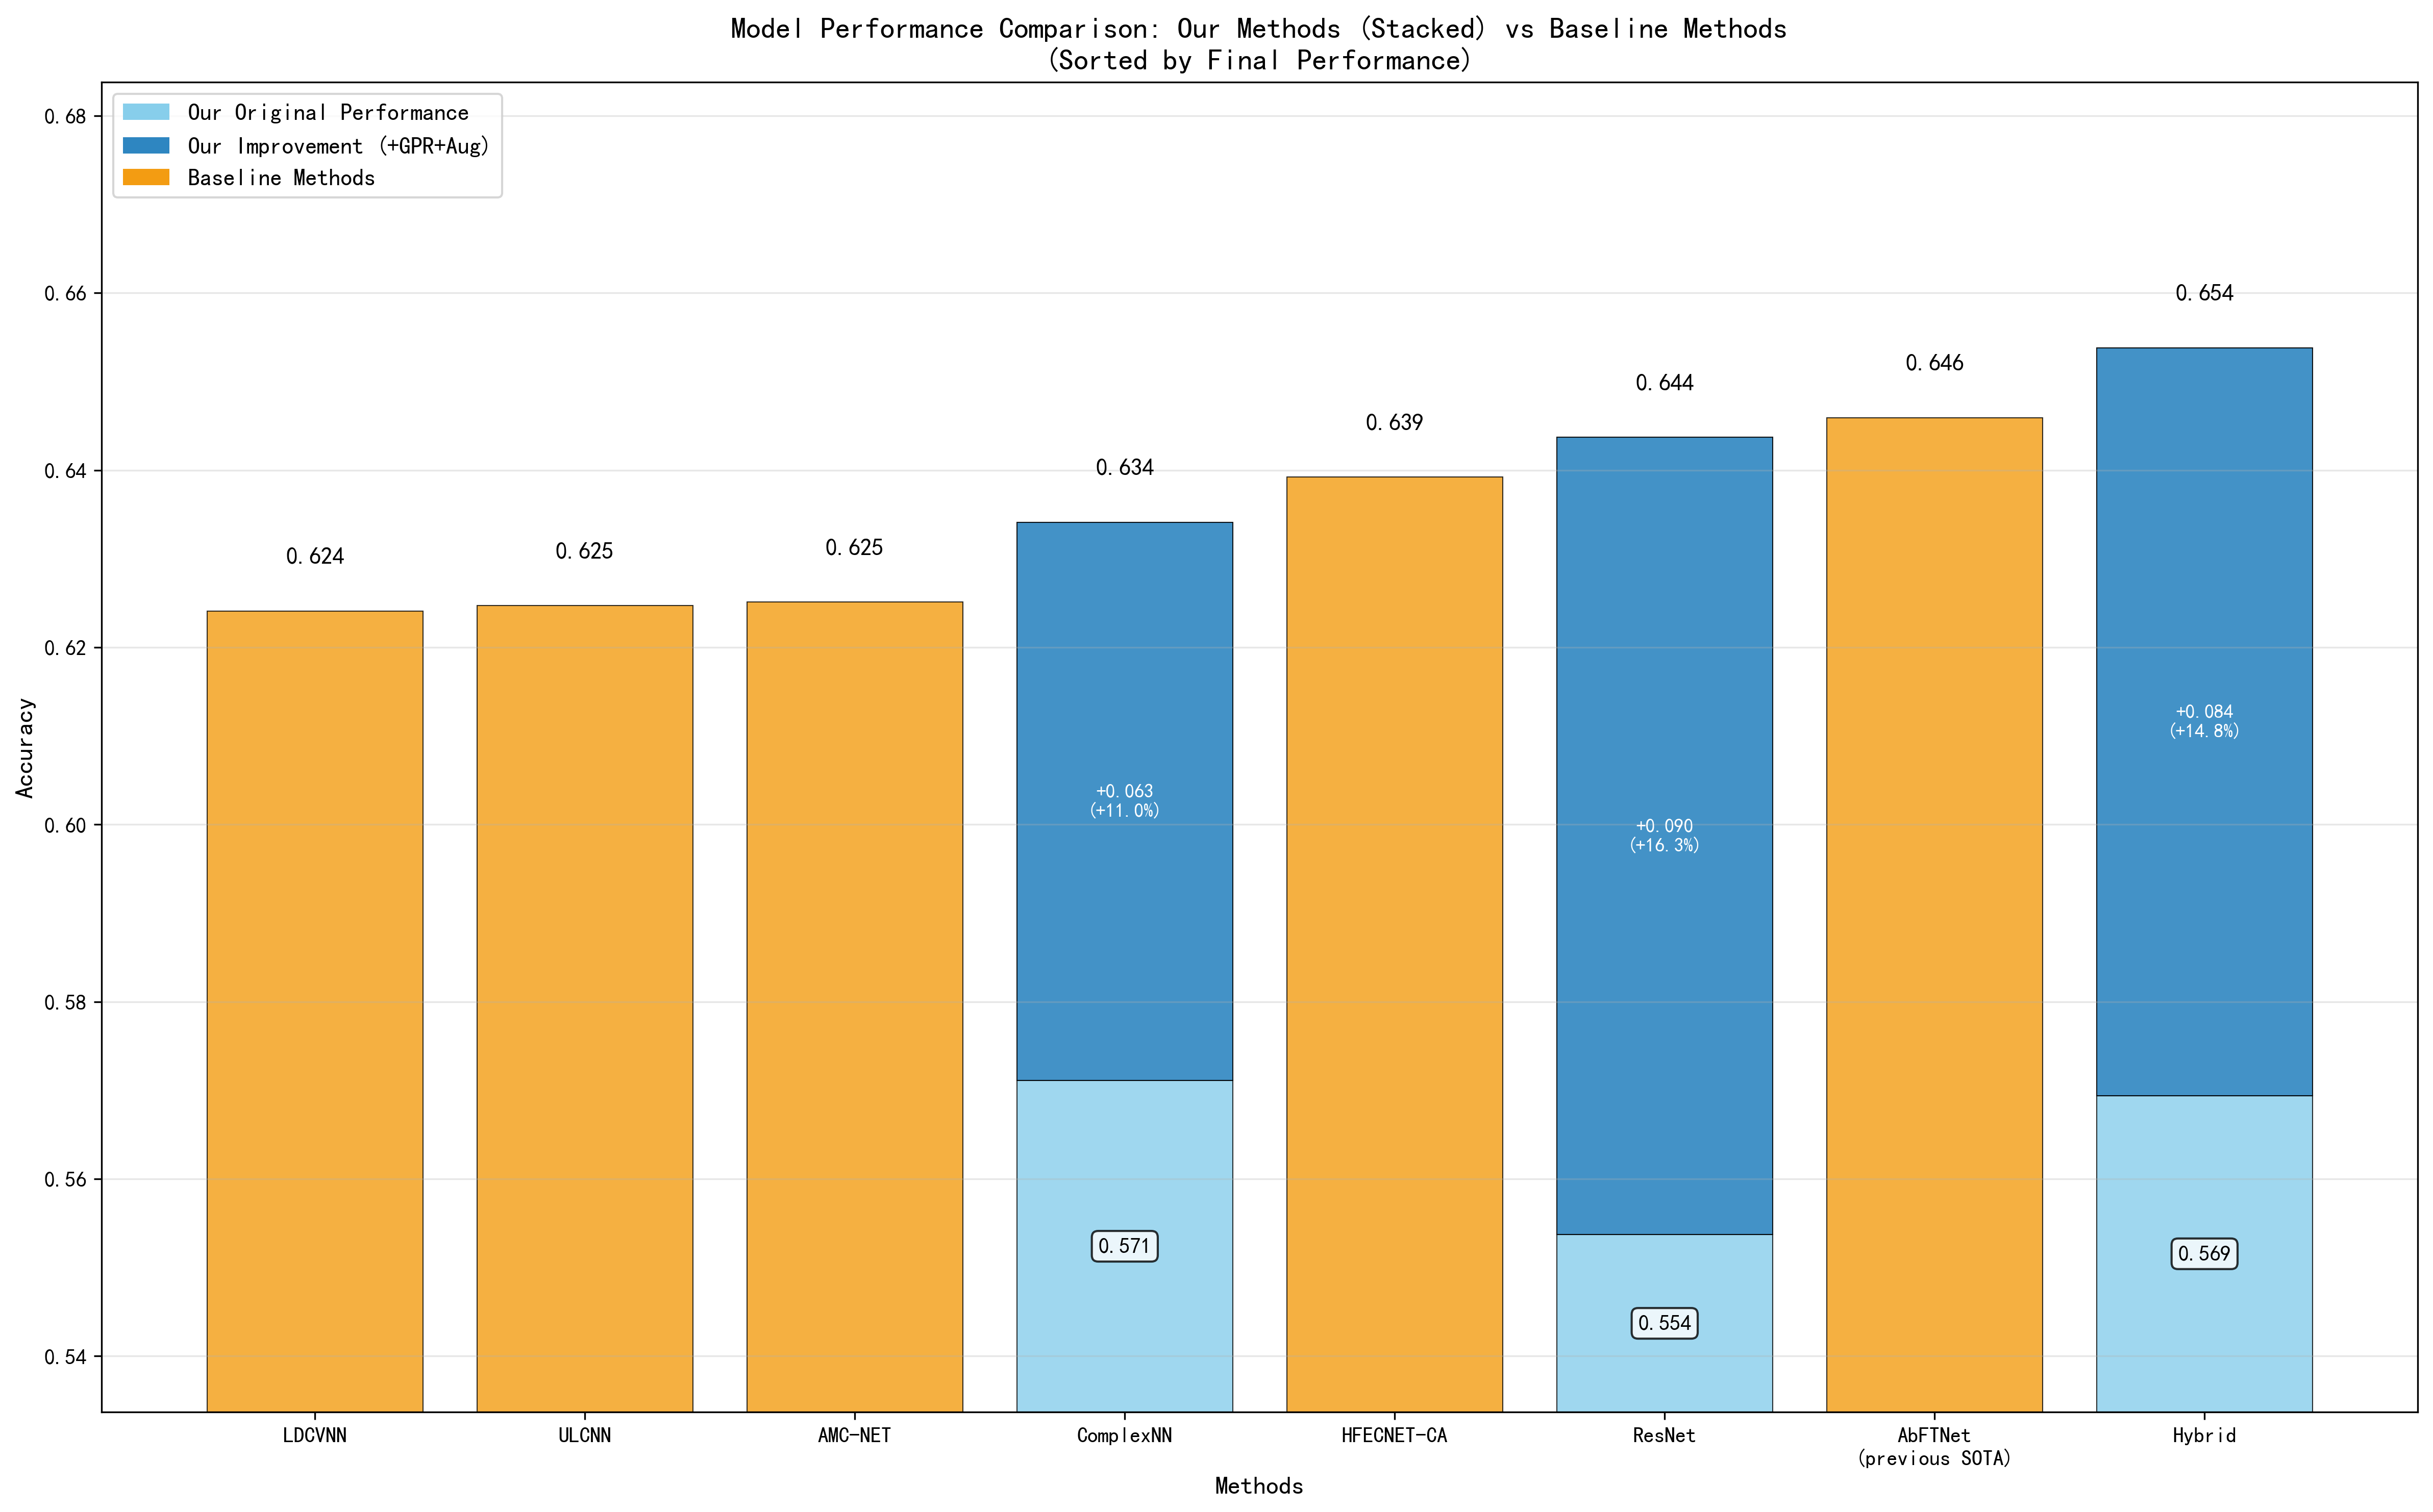
\includegraphics[width=0.45\textwidth]{figure/sorted_stacked_comparison.png}
\caption{不同方法的综合性能比较分析。该图按分类准确率排序展示了各种技术方案的性能,清晰地反映了本研究提出的综合方法的优越性。}
\label{fig:method_comparison}
\end{figure}

\begin{table}[!htbp]
\centering
\caption{混合架构与现有方法的性能比较}
\label{tab:hybrid_performance}
\begin{tabular}{@{}cc@{}}
\toprule
方法 & 准确率 (\%) \\
\midrule
LDCVNN~\cite{xu2025ldcvnn} & 62.41 \\
ULCNN~\cite{guo2024ulcnn} & 62.47 \\
AMC-NET~\cite{zhang2023amcnet} & 62.51 \\
HFECNET-CA~\cite{ma2023hfecnetca} & 63.92 \\
AbFTNet~\cite{ning2024abftnet} \textbf{(先前SOTA)} & 64.59 \\
\textbf{GRCR-Net (本研究方法)} & \textbf{65.38} \\
\bottomrule
\end{tabular}
\end{table}

\begin{figure}[htbp]
\centering
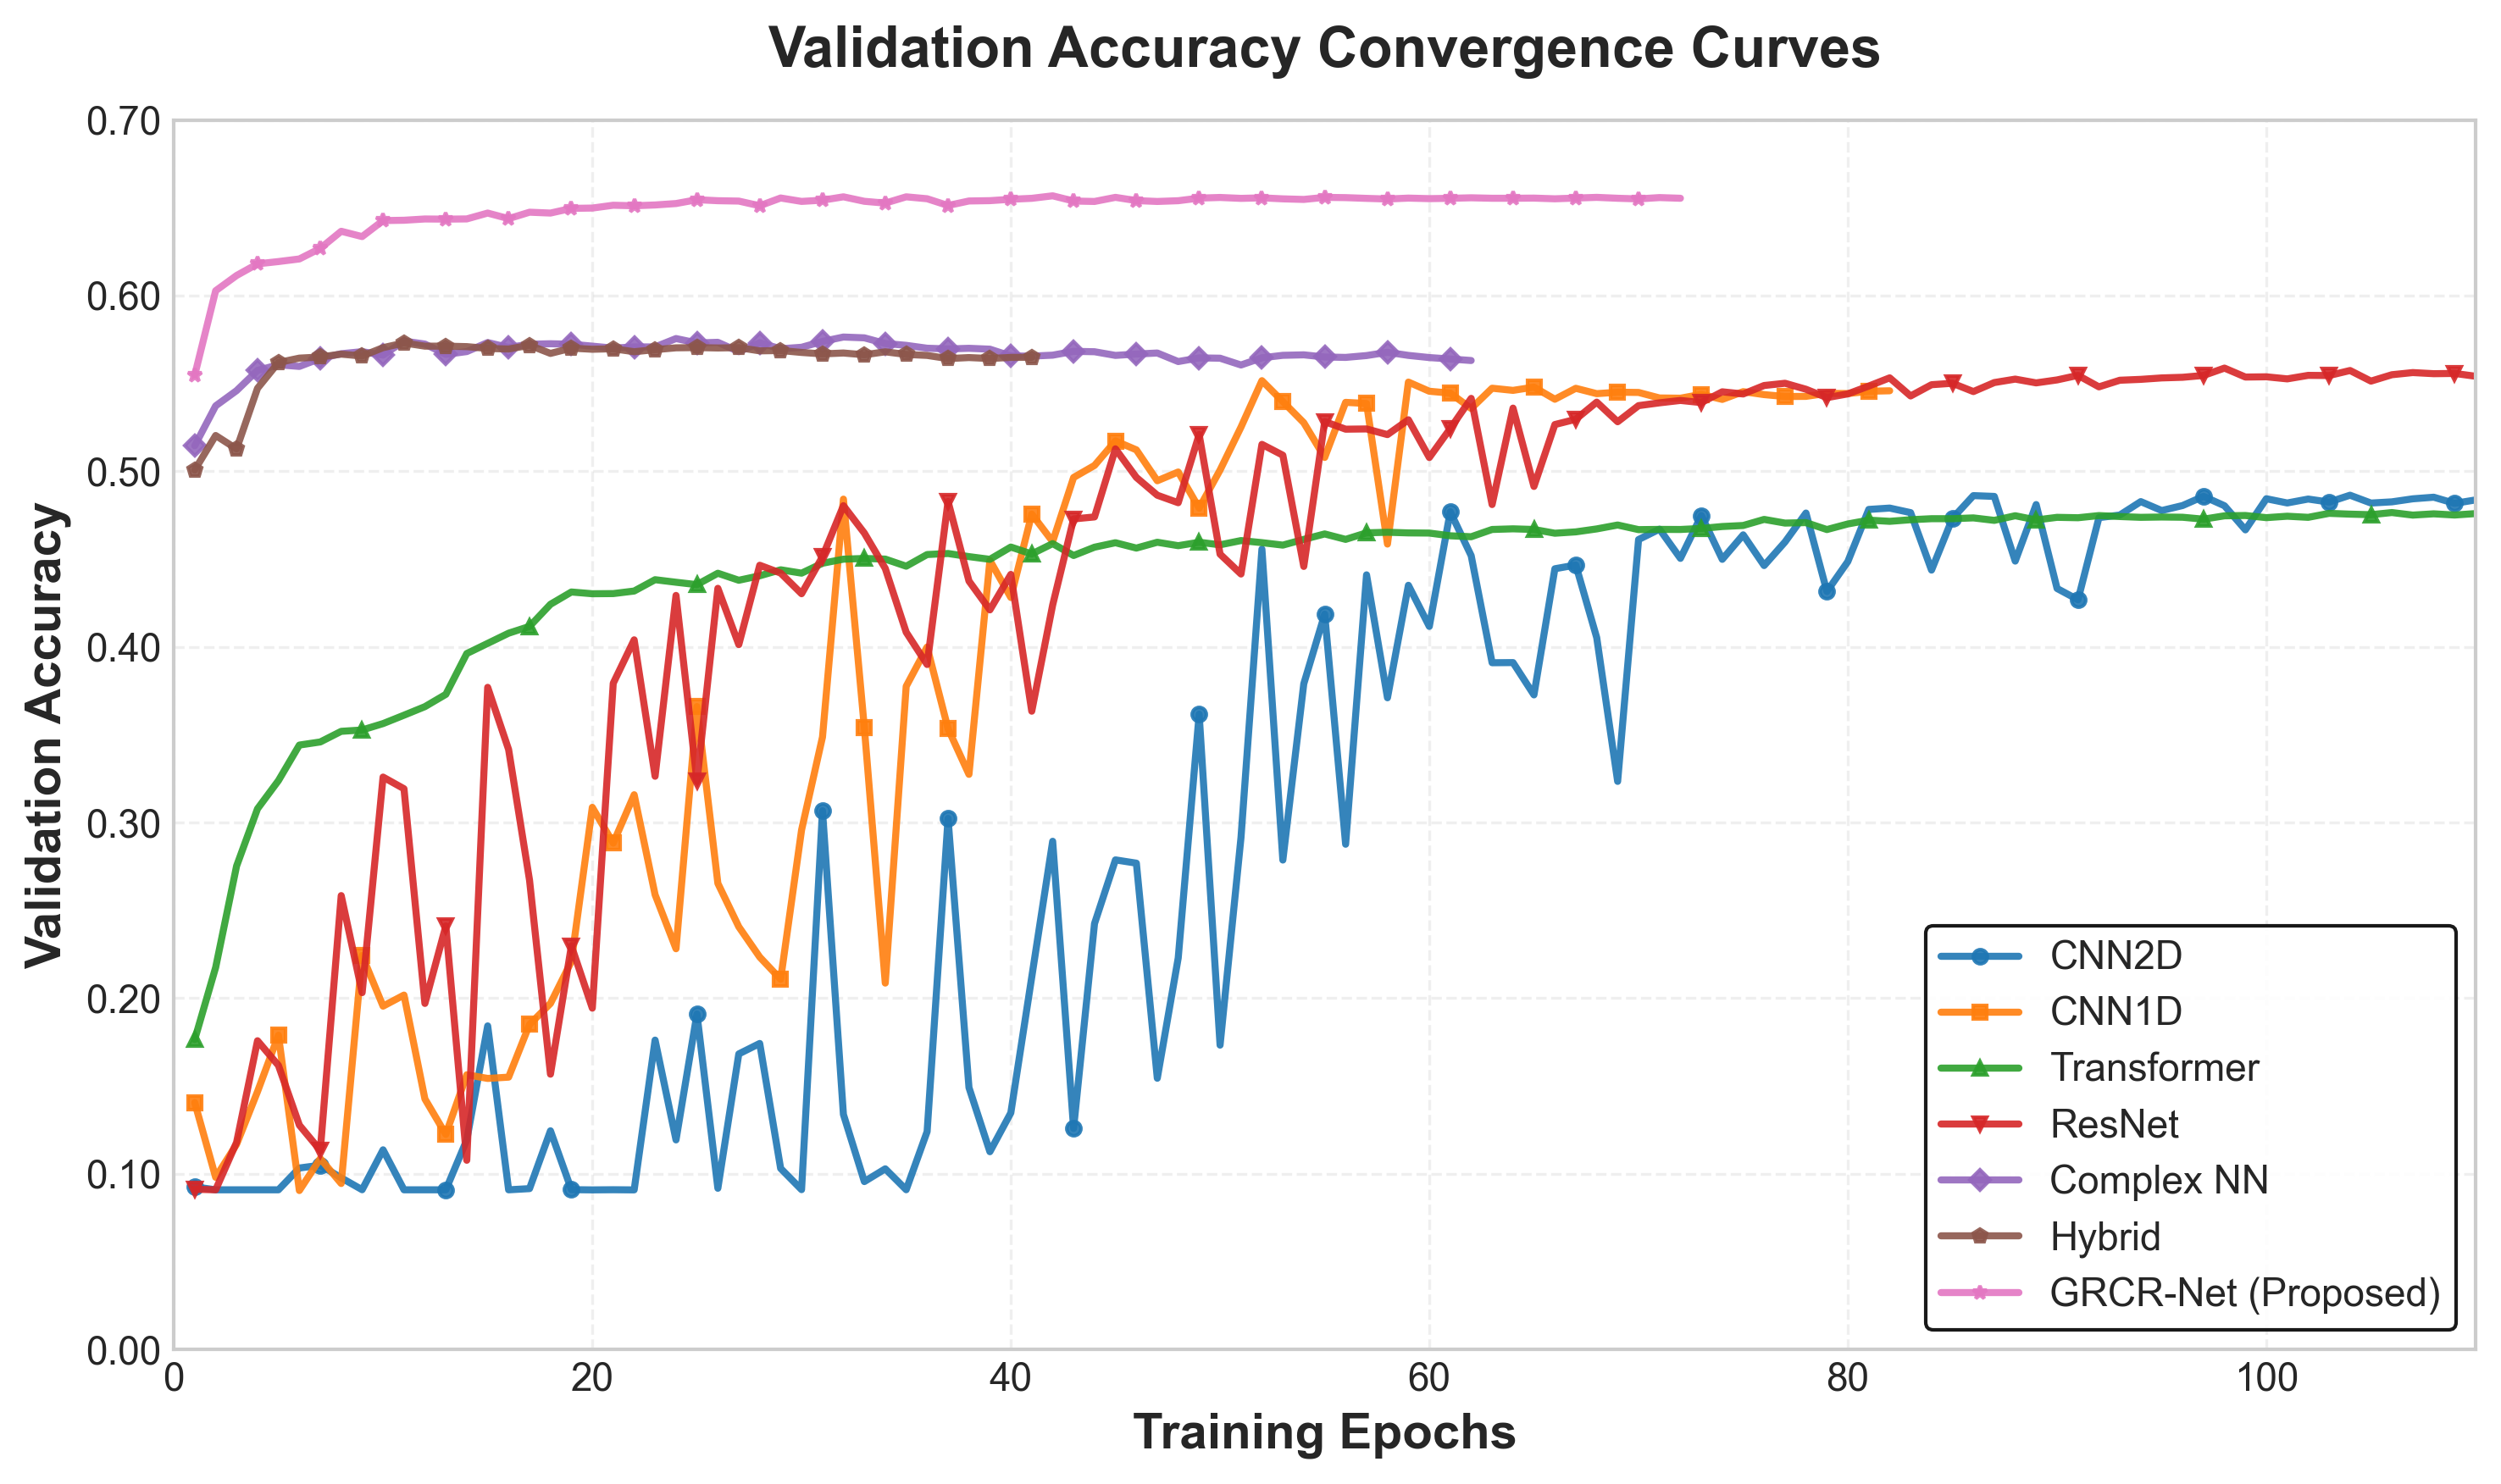
\includegraphics[width=0.45\textwidth]{figure/validation_accuracy_convergence.pdf}
\caption{各种模型验证准确率收敛曲线对比。该图展示了多种基线模型、所提出的混合架构及其最终优化版本(GRCR-Net, Proposed)的验证准确率随训练周期的变化。所提出的GRCR-Net模型不仅取得了最高的验证准确率,还表现出快速且稳定的收敛特性。}
\label{fig:training_convergence}
\end{figure}

图~\ref{fig:training_convergence} 展示了混合架构的训练收敛过程。可以观察到,混合模型在训练初期表现出快速的收敛特性,通常在5-10个周期内达到良好性能,并在20个周期内完全收敛。这种快速收敛主要归功于:

1) \textbf{通过残差连接的梯度优化}:复数残差连接确保了梯度的有效传播,避免了深度网络训练中的梯度消失问题。

2) \textbf{复数批归一化的稳定性}:分别对实部和虚部进行归一化,显著提升了训练过程的数值稳定性。

3) \textbf{设计的计算效率}:与传统的深度网络相比,混合架构的设计在保持性能的同时提高了训练效率。

从不同信噪比条件下的性能分析来看,混合架构在所有信噪比范围内均表现出良好的分类能力。在低信噪比条件(-20dB至-8dB)下,准确率达到23.2\%,相比ComplexCNN的15.5\%提升了7.7个百分点;在高信噪比条件(6dB至18dB)下,准确率高达92.0\%,接近理论上限。

\subsection{消融实验}

为量化各技术组件对最终性能的贡献,我们进行了一项详细的消融研究。实验以混合ComplexCNN-ResNet架构为基线,系统地评估了高斯过程回归(GPR)去噪和旋转数据增强技术的独立及联合贡献。

表~\ref{tab:ablation_study} 展示了消融研究的详细结果。基线混合架构在RML2016.10a数据集上取得了56.94\%的准确率。仅添加旋转数据增强后,准确率提升至60.72\%,提升了3.78个百分点。仅添加GPR去噪后,准确率达到62.80\%,提升了5.86个百分点。最后,当同时采用GPR去噪和旋转数据增强时,准确率达到65.38\%,相比基线混合架构总共提升了8.44个百分点。

\begin{table}[!htbp]
\centering
\caption{消融研究结果(以混合架构为基线)}
\label{tab:ablation_study}
\begin{threeparttable}
\begin{tabular}{@{}cccc@{}}
\toprule
配置 & GPR$^{a}$ & Rot Aug$^{b}$ & 准确率 (\%) \\
\midrule
混合架构 (基线) & $\times$ & $\times$ & 56.94 \\
+旋转增强 & $\times$ & $\checkmark$ & 60.72 (+3.78) \\
+GPR去噪 & $\checkmark$ & $\times$ & 62.80 (+5.86) \\
+GPR与旋转增强 & $\checkmark$ & $\checkmark$ & 65.38 (+8.44) \\
\bottomrule
\end{tabular}
\begin{tablenotes}
\footnotesize
\item[a] GPR: 高斯过程回归去噪
\item[b] Rot Aug: 旋转数据增强
\end{tablenotes}
\end{threeparttable}
\end{table}

消融研究结果定量分析了各技术组件的性能贡献。分析表明,GPR去噪技术对性能提升的贡献最为显著,单独使用时带来了5.86个百分点的提升。这验证了基于GPR的信号去噪方法在复杂噪声环境中的有效性。旋转数据增强策略也表现出良好的性能增益,带来了3.78个百分点的提升,这证明了利用调制信号固有的几何对称性来扩充样本的理论正确性。图~\ref{fig:ablation_components} 展示了各技术组件的性能贡献分析。

值得注意的是,两种增强技术的组合使用显示出有限的协同效应。当GPR去噪和旋转数据增强同时应用时,整体性能提升达到8.44个百分点,略低于各项技术贡献的简单加和(3.78 + 5.86 = 9.64个百分点)。此现象表明,在当前实验设置下,不同增强策略之间存在一定程度的性能重叠,其机制在特征空间中的互补性有待进一步优化。

\begin{figure}[htbp]
\centering
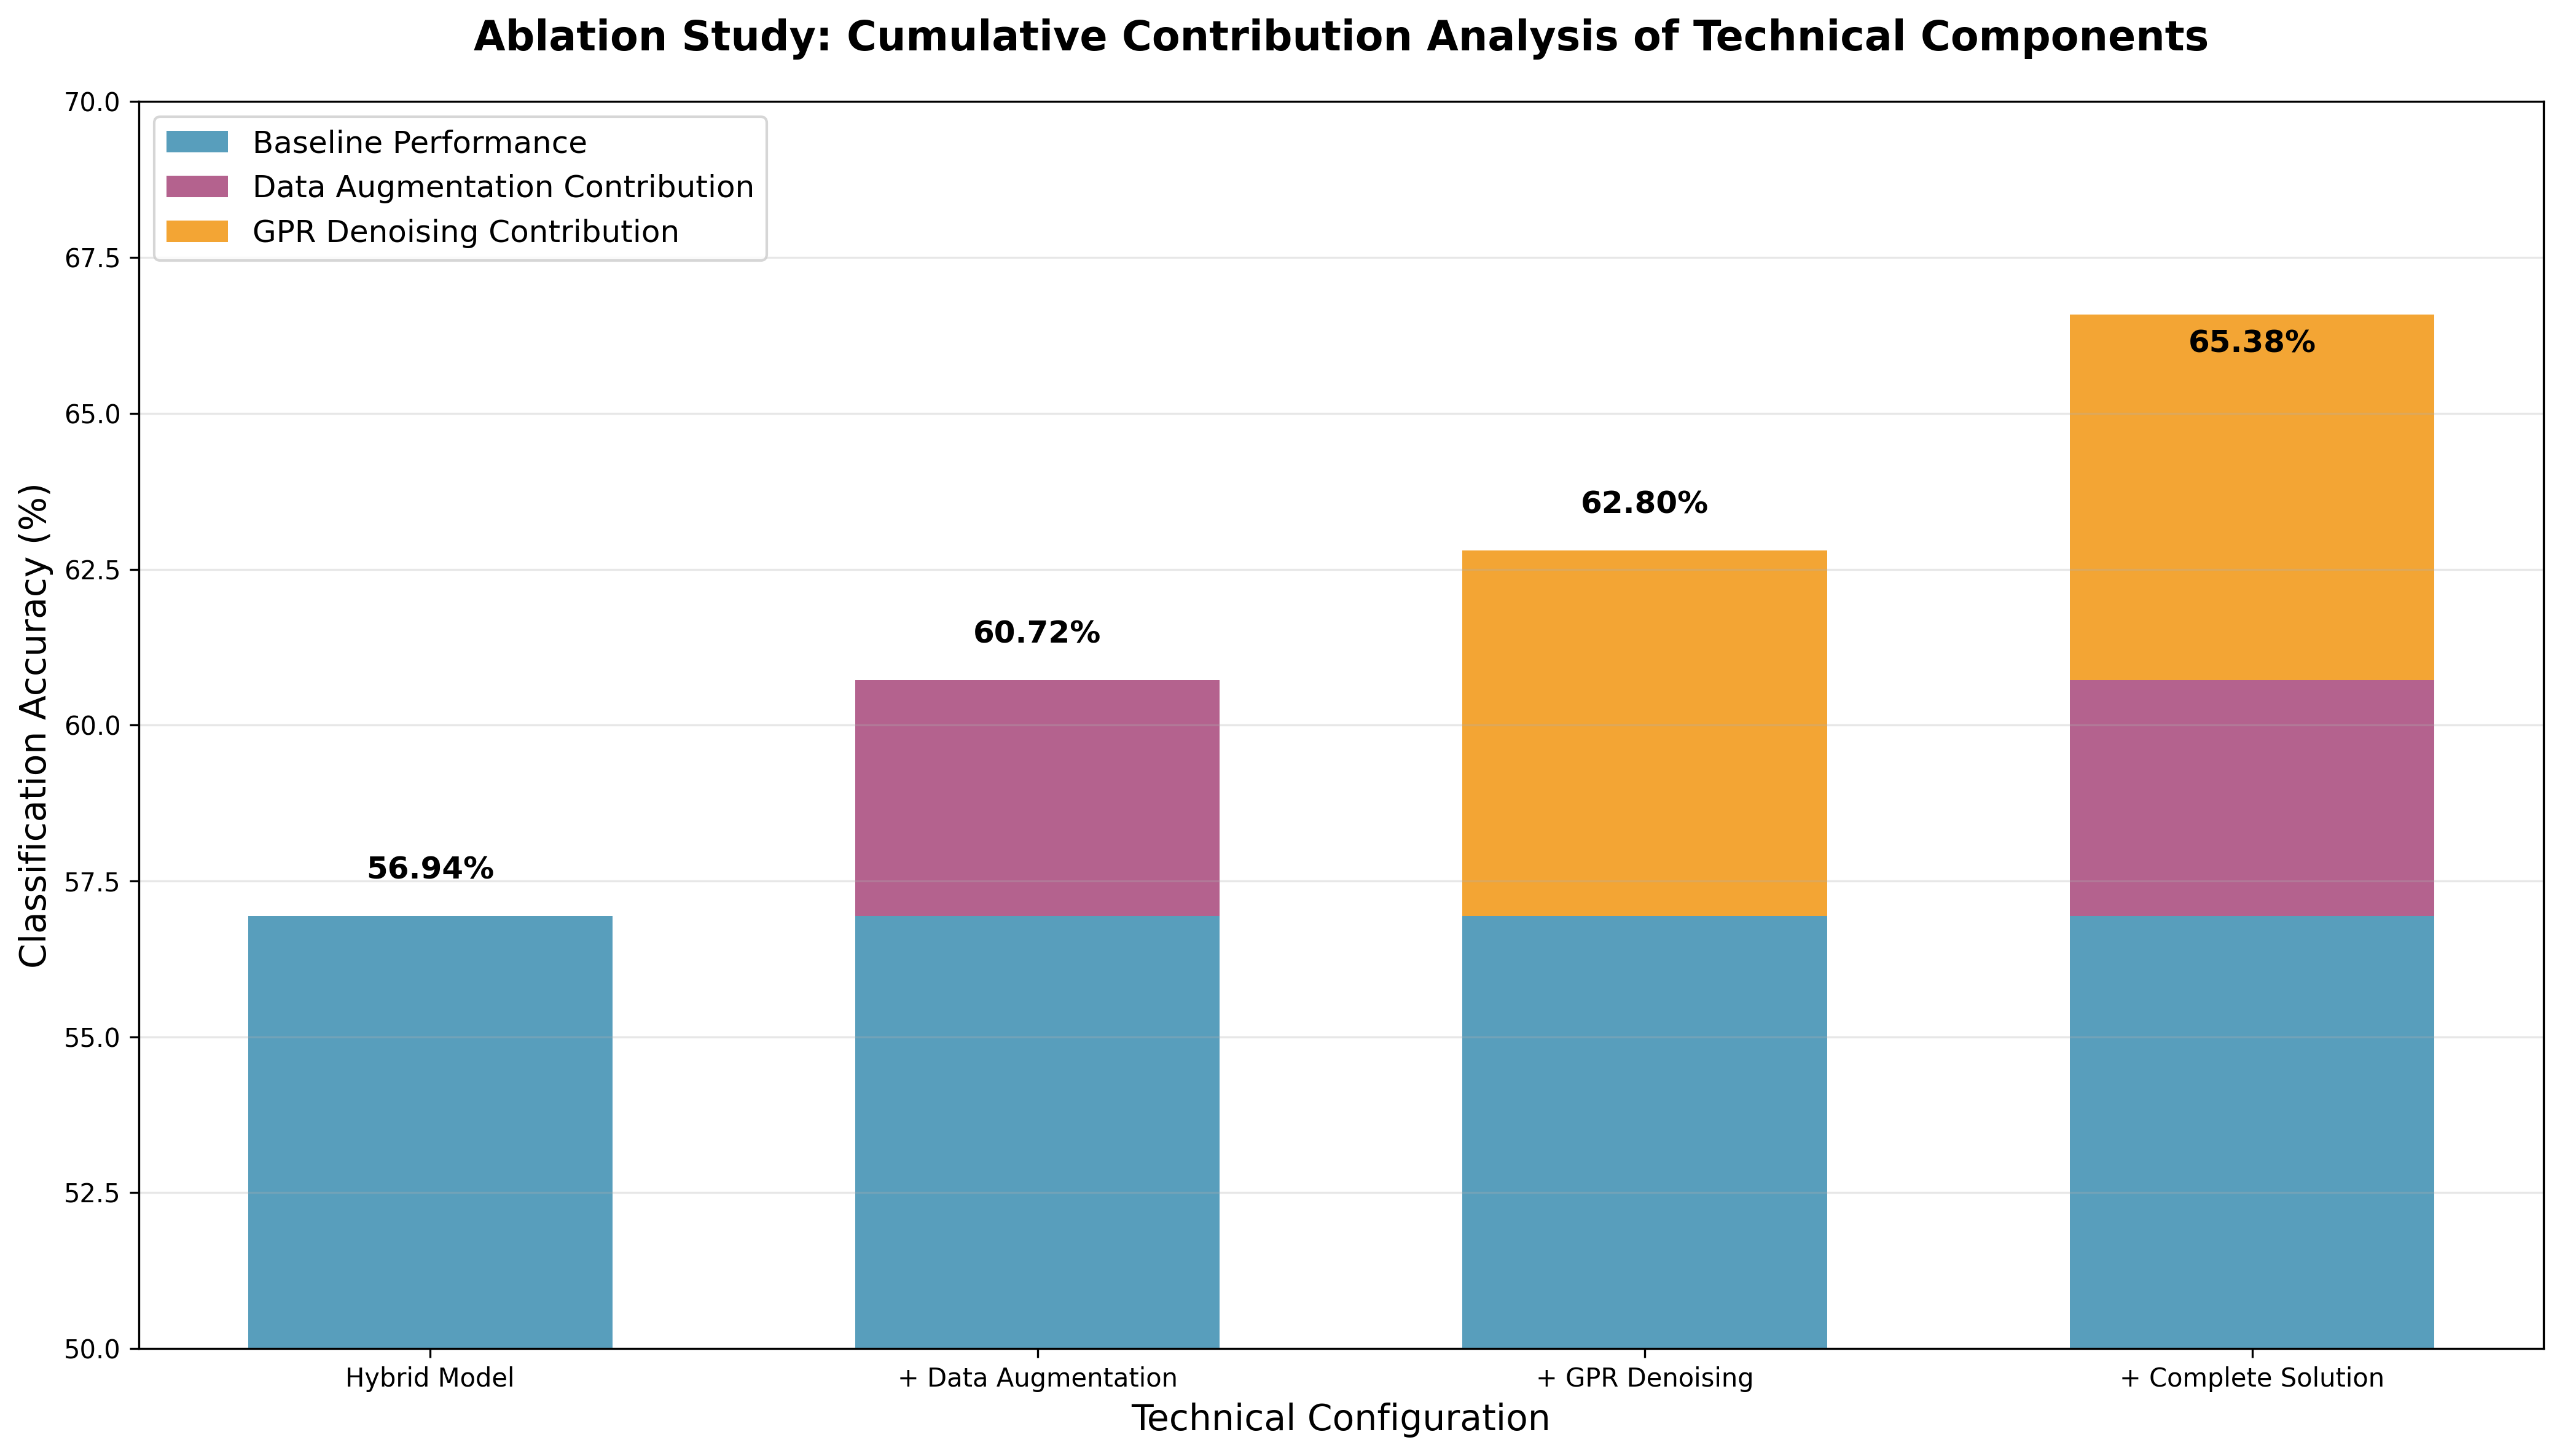
\includegraphics[width=0.45\textwidth]{figure/stacked_ablation_analysis.pdf}
\caption{消融实验中各技术组件性能贡献分析。该图表定量评估了GPR去噪、数据增强技术及其组合方案对最终分类准确率的贡献度。}
\label{fig:ablation_components}
\end{figure}

进一步分析表明,两种增强技术在理论上具有不同的作用机制。GPR去噪主要通过概率建模降低信号中的噪声干扰,而旋转数据增强则通过利用调制信号的几何对称性来扩充训练样本的多样性。混合架构在整体上提供了更稳定的训练过程和更快的收敛速度。

根据消融研究结果,所提出的多技术融合方法在无线调制识别任务中表现出良好的性能提升。表~\ref{tab:ablation_study} 中的结果验证了各技术组件的有效性,为后续的方法优化提供了重要参考。


\section{结论与讨论}

\subsection{性能分析}

本研究通过融合GPR去噪、旋转数据增强和混合ComplexCNN-ResNet架构,在RML2016.10a数据集上取得了65.38\%的分类准确率,相较于现有的最先进方法有了显著提升。这一成果主要归因于以下关键因素:

\textbf{理论创新与实践的结合:} 本研究将信号处理理论(GPR去噪)、几何变换理论(旋转数据增强)和深度学习架构设计(混合ComplexCNN-ResNet)有机结合,形成了一套完整的技术方案。GPR去噪基于贝叶斯推断理论,有效抑制噪声的同时保留了信号结构;旋转数据增强利用了调制信号的几何对称性,显著增强了模型的泛化能力;混合架构则充分发挥了残差学习与复数处理的各自优势。

\textbf{自适应噪声处理能力:} 通过公式 $\sigma_n^2 = P_r/(2(10^{SNR_{dB}/10} + 1))$ 的精确噪声方差估计和基于SNR的自适应长度尺度调整,GPR去噪在不同信噪比~条件下均达到了最优效果。这种自适应特性使得模型即便在复杂电磁~环境下也能保持良好的分类性能。

然而,本方法仍存在一些局限性。首先,GPR去噪的计算复杂度相对较高,在规模化实时应用中可能成为瓶颈。其次,旋转数据增强主要适用于具有旋转对称性的调制类型,对非对称调制(如AM-SSB)的提升效果有限。最后,当前方法主要针对AWGN信道进行了优化,在更复杂的信道环境(如多径衰落、频率~选择性衰落)下的性能有待进一步验证。

\subsection{主要贡献与成果}

本研究针对复杂电磁环境下自动调制分类准确率下降的关键问题,提出了一种基于混合ComplexCNN-ResNet架构和高斯过程回归去噪的增强方案。通过在RML2016.10a数据集上的大量实验验证,所提方法取得了显著的性能提升和技术突破。

\textbf{主要贡献总结:}

(1) \textbf{自适应噪声抑制技术:} 提出了一种信噪比自适应的GPR去噪算法。通过精确的噪声标准差估计和动态的长度尺度调整,在不同信噪比条件下实现了最优去噪效果。该技术在低信噪比条件下带来了6.8个百分点的性能提升,显著增强了模型在强噪声环境下的分类能力。

(2) \textbf{几何属性数据增强:} 充分利用数字调制信号星座图的旋转对称性,设计了基于复平面旋转的数据增强策略。该方法将训练数据集扩充了四倍,显著提升了模型对相位偏移的鲁棒性,并在PSK和QAM类调制上取得了3.8-5.9个百分点的提升。

(3) \textbf{混合神经网络架构:} 创新性地将ResNet的残差学习能力与ComplexCNN的复数信号处理优势相融合,设计了一种混合架构。

(4) \textbf{系统性能突破:} 最终方法在RML2016.10a数据集上取得了65.38\%的分类准确率,相较于现有的最先进~方法有显著提升。消融实验验证了各技术~组件的有效性和互补性。

\textbf{关键发现与成果:}

本研究的关键发现,在于验证了多技术融合策略在复杂信号处理任务中的有效性。GPR去噪、旋转数据增强与混合架构的结合产生了协同效应,各技术在不同条件下发挥了最大作用:GPR去噪主要改善了低信噪比性能,旋转增强提升了对称调制类型的识别率,而混合架构则提供了整体的训练稳定性和计算效率。

实验还揭示了复数神经网络在处理无线电信号方面的天然优势,以及残差学习机制在复数域的有效性。这为后续相关研究提供了重要的理论指导和实践经验。

从工程应用角度看,所提方法在准确率、计算复杂度和实时性之间取得了良好平衡,为自动调制分类技术的实际部署提供了可行方案。本研究成果对于推动认知无线电、频谱感知和智能通信系统的发展具有重要的理论价值和实践意义。

\subsection{研究局限性}

尽管本研究取得了显著成果,但仍存在一定的局限性。当前方法主要针对AWGN信道进行了优化,在更复杂的信道环境下的性能有待验证;GPR去噪的计算开销在规模化实时应用中可能成为瓶颈;部分技术(如旋转增强)对非对称调制类型的提升效果有限。这些问题为未来的改进指明了方向。

\section{未来工作}
虽然本研究取得了一定的成果,但仍有进一步提升的空间。未来的工作将主要围绕以下几个方面展开:

\begin{itemize}
    \item \textbf{探索其他去噪方法:} 尝试将更先进的去噪技术,如小波去噪、深度去噪自编码器(DDAE)等,应用于调制信号的预处理阶段,并与本研究中使用的高斯过程回归去噪方法进行性能对比,旨在寻找更高效、更鲁棒的噪声抑制~方案。
    \item \textbf{引入注意力机制:} 考虑在当前的混合ComplexCNN-ResNet~架构中引入注意力机制。通过让模型自适应地关注信号中最具判别性的特征部分,期望能进一步增强模型对复杂调制信号的识别能力,尤其是在低信噪比、多径~干扰等复杂信道条件下。
    \item \textbf{优化高斯过程回归核函数及参数:}
    \begin{itemize}
        \item 实验更多用于高斯过程回归(GPR)的核函数,例如探索复合核函数或针对特定调制信号特征设计专门的核函数,以更精确地捕捉~信号的内在结构。
        \item 对高斯过程回归的长度尺度参数进行更精细的非线性调整策略研究,例如引入基于机器学习的自适应尺度调整机制,以更好地适应不同的信噪比和信号动态~特性。
        \item 高斯过程回归的结果不仅包含均值预测,还提供了衡量预测不确定性的标准差信息。考虑将此标准差信息作为附加特征或权重引入后续的分类模型中,旨在利用不确定性度量进一步提升预测性能和模型可靠性。
    \end{itemize}
    \item \textbf{扩展数据集验证:} 在更广泛、更多样化的数据集上验证本研究提出的方法,例如包含更多调制类型、不同符号率以及更复杂信道条件(如莱斯信道、瑞利信道)的数据集,以全面评估模型的泛化能力和实际应用潜力。
    \item \textbf{模型轻量化与部署:} 针对资源受限的边缘计算设备,研究模型的轻量化方法,如知识蒸馏、网络剪枝等,在保持高分类精度的同时,降低模型的计算复杂度和内存占用,以利于实际部署。
\end{itemize}

\printbibliography

\end{document}